\documentclass[14pt, a4paper]{extreport}
	\usepackage[left=25mm, right=10mm, top=20mm, bottom=20mm]{geometry}
	\usepackage[hidelinks, linktoc=all, pagebackref]{hyperref}
	\usepackage{indentfirst}
    \usepackage{subcaption}
   	\usepackage[biblabel]{cite}
    \usepackage[font=small,labelfont=bf]{caption}
    \usepackage{abstract}
    \usepackage{mathtools}
    \usepackage[russian]{babel}
    \usepackage{mathrsfs}  
    \usepackage{fontawesome}
    \usepackage{cleveref}
    \usepackage{fancyhdr}
    \usepackage{qrcode}
    \usepackage{enumitem}
    \setlength{\parskip}{0.1cm}   
	\setlength{\parindent}{0.7cm}
	\usepackage{setspace}
	\onehalfspacing
    \usepackage{graphicx} % Used to insert images
    \usepackage{adjustbox} % Used to constrain images to a maximum size 
   	\usepackage{color} % Allow colors to be defined
    \usepackage{amsmath} % Equations
    \usepackage{amssymb} % Equations
    \usepackage[mathletters]{ucs} % Extended unicode (utf-8) support
    \usepackage[utf8x]{inputenc} % Allow utf-8 characters in the tex document
    \usepackage{fancyvrb} % verbatim replacement that allows latex
    \usepackage{grffile} 
    \usepackage{tabularx}
	\usepackage{bbm}
	
	\usepackage{tocloft}
	\renewcommand\cftsecleader{\cftdotfill{\cftdotsep}}
	\renewcommand{\cftchapleader}{\cftdotfill{\cftdotsep}}


	\usepackage{titlesec}
	
	\titleformat{\chapter}
	{\normalfont\fontsize{20}{24}\bfseries}{\thechapter}{1em}{}
	
	
	\titleformat{\section}
	{\normalfont\fontsize{16}{20}\bfseries}{\thesection}{1em}{}
	\titleformat{\subsection}
	{\normalfont\fontsize{14}{16}\bfseries}{\thesubsection}{1em}{}

\newcommand{\diff}{\,\mathrm{d}} 	
 \renewcommand{\figureautorefname}{Рис.}%
\renewcommand*\thesection{\arabic{section}}
\DeclarePairedDelimiter\bra{\langle}{\rvert}
\DeclarePairedDelimiter\ket{\lvert}{\rangle}
\DeclarePairedDelimiterX\braket[2]{\langle}{\rangle}{#1 \delimsize\vert #2}
\newcommand{\rbrkt}[1]{\left( #1 \right)}
\newcommand{\sbrkt}[1]{\left[ #1 \right]}
\newcommand{\rot}{\text{\textbf{rot}}\,}

\renewcommand*{\backreftwosep}{ and~}
\renewcommand*{\backreflastsep}{ and~}
\renewcommand*{\backref}[1]{}
\renewcommand*{\backrefalt}[4]{%
\ifcase #1 %
\relax%
\or
(referenced on p. [#2])%
\else
(referenced on p. [#2])%
\fi
}

\numberwithin{equation}{section}
\setcounter{tocdepth}{3}


\renewcommand*\thesection{\arabic{chapter}.\arabic{section}}
\lhead[\rm\thepage]{\fancyplain{}{\nouppercase{\sl{\rightmark}}}}
\rhead[\fancyplain{}{\nouppercase{\sl{\leftmark}}}]{\rm\thepage}
\chead{}\lfoot{}\rfoot{}\cfoot{}
\pagestyle{plain}


\graphicspath{{Pictures/}}


\begin{document}

\selectlanguage{russian}
\begin{titlepage}
\par 
\vspace*{-2cm}
\begin{center}
Министерство образования и науки Российской Федерации\\
Федеральное государственное автономное образовательное учреждение высшего\\ 
профессионального образования \\
<<Московский физико-технический институт (государственный университет)>> 
\end{center}

\vspace*{0.2cm}
\begin{flushright}
На правах рукописи\\
УДК 539.12
\end{flushright}

\vfill

\begin{center}
Федоров Глеб Петрович

\vspace*{0.5cm}

{\large Моделирование квантового взаимодействия излучения и вещества с использованием массивов сверхпроводниковых искусственных атомов}


\begin{center}
Специальность 03.04.01 ---\\ <<Прикладные математика и физика>>\\
\vspace{0.5cm}
Диссертация на соискание учёной степени \\
кандидата физико-математических наук
\end{center}


\vspace*{2cm}


\begin{flushright}
Научный руководитель\\
д. ф.-м. н., проф.\\
Рязанов Валерий Владимирович
\end{flushright}



\vfill

Москва

2021 г. 
\end {center} 
\end{titlepage}


\tableofcontents

\chapter*{Введение}
\addcontentsline{toc}{chapter}{Введение} 

\section*{Актуальность работы}

История развития сверхпроводниковых искусственных атомов, или кубитов, как инструмента для наблюдения макроскопических квантовых эффектов берет своё начало в 1997 году, когда в группе проф. Накамуры в Японии была впервые показана \cite{nakamura1997spectroscopy} когерентность суперпозиции зарядовых состояний одноэлектронного транзистора. Этот эксперимент стал толчком к развитию новой области физики, интерес к которой обеспечивался как открывшимися возможностями изучать фундаментальные физические явления, так и потенциальной применимостью для квантовых вычислений.

Несмотря на относительно недавнее появление, сверхпроводниковые, или джозефсоновские кубиты, как их также называют, прошли много стадий в своем развитии. Системы, использовавшиеся в первых экспериментах, имели очень низкие времена когерентности: например, в работе \cite{nakamura1999coherent} время затухания Раби-осцилляций в зарядовом кубите составило около 1 нс, в то время как сейчас рекордные времена когерентности составляют порядка 100 микросекунд \cite{kjaergaard2020superconducting}. Наиболее далеко в области квантовых вычислений продвинулись американские учёные, работающие теперь в компаниях Google и IBM. В частности, в 2019 году Google продемонстрировали \cite{arute2019quantum} квантовое превосходство своего процессора из 53 кубитов над мощнейшим существующим классическим компьютером. Однако даже этот результат пока ещё далёк от реальных практических применений, так как количество ошибок, происходящих в устройстве, пока еще очень велико, и решаемая задача была создана искусственно для минимизации чувствительности результата к декогеренции. Как было показано еще Шором в ХХ веке \cite{shor1995scheme}, практические квантовые вычисления потребуют реализации алгоритмов коррекции ошибок, что неминуемо требует существенного увеличения числа физических кубитов, требующихся для обеспечения работы небольшого числа логических. Увеличение числа кубитов более, чем на порядок, непременно натолкнётся на трудности масштабирования контролирующей электроники и криогенной аппаратуры \cite{krinner2019engineering}, алгоритмов калибровки системы \cite{arute2019quantum, kelly2018physical}, а также проектирования самих сверхпроводящих интегральных схем \cite{hutchings2017tunable}. Отсюда следует, что сегодня нельзя назвать даже примерных сроков реализации полезных квантовых алгоритмов \cite{arute2019quantum}.

Однако острый интерес к потенциальным применениям в области квантовых вычислений помог мотивировать исследования со сверхпроводящими кубитами и по другим направлениям \cite{kjaergaard2020superconducting}. В частности, чрезвычайно большое количество экспериментов было проведено в области квантовой электродинамики цепей \cite{blais2020quantum}, вдохновленной нобелевскими исследования Гароша \cite{haroche2013nobel} по стандартной квантовой электродинамике полостей. Впервые сверхпроводниковый искусственный атом был сильно связан (strongly coupled) с квантованным полем в резонаторе в 2004 году в Йельском университете \cite{wallraff2004strong}, что стало первым в истории экспериментальным подтверждением возможности связать одиночную квантовую систему с полем так, чтобы сила связи превысила диссипацию. С развитием технологии производства алюминиевых сверхпроводниковых чипов, открытием новых схем расположения их элементов, а также удешевлением электроники все больше групп в мире стали включаться в работу и вести собственные исследования. В Йельском университете работают проф. Деворе (Michel Devoret) и проф. Шелькопф (Robert Schoelkopf), занимающиеся в основном экспериментами с неклассическими состояниями света в микроволновых резонаторах, которые они готовят, используя связанные с ними искусственные атомы (см. \cite{vlastakis2013deterministically, mirrahimi2014dynamically}). В этой группе также берут начало известные работы компании IBM (см. \cite{jurcevic2020demonstration}), а также стартапа Rigetti, по фамилии одного из защитившегося в Йеле аспирантов \cite{reagor2018demonstration}. В группе проф. Мартиниса (John Martinis) в университете Калифорнии, Санта Барбара, помимо обширной работы по развитию квантовых алгоритмов \cite{arute2019quantum}, проводились исследования многочастичной локализации \cite{chen2014emulating, roushan2017spectroscopic}, квантового хаоса. В группе проф. Сиддики (Irfan Siddiqi), университет Калифорнии, Бёркли, проводятся эксперименты по наблюдению и изучению отдельных квантовых траекторий и квантовых скачков, которые испытывает кубит под воздействием сильных или слабых измерений (см. \cite{hacohen2016quantum} и ссылки там же). Проф. Астафьев, работавший в Японии и затем в Англии, провёл первые эксперименты по взаимодействию свободного излучения в волноводах с джозефсоновскими кубитами \cite{astafiev2010resonance}. В Дельфтском университете под руководством проф. Ди Карло (Leonardo Di Carlo) проводились одни из первых экспериментов по реализации квантовых алгоритмов на двухкубитных схемах, а затем изучалась возможность цифрового моделирования произвольных гамильтонианов \cite{langford2017experimentally}. Наконец, в группе проф. Волрафа (Andreas Wallraff) проводятся эксперименты с одиночными микроволновыми фотонами, например, по созданию источника последовательности перепутанных друг с другом фотонов \cite{besse2020realizing} или использовать одиночные летящие фотоны для перепутывания удаленных кубитов \cite{kurpiers2018deterministic}.

Как можно видеть, с течением времени обнаружился обширный перечень областей применения сверхпроводниковых квантовых систем, без которых все приведенные выше эксперименты были бы невозможны. Исследования, описанные в данной диссертации, посвящены экспериментальной реализации взаимодействия излучения и вещества в квантовом режиме при помощи сверхпроводниковых искусственных атомов. Данная тема лежит за пределами области цифровых квантовых вычислений и скорее оказывается ближе к аналоговому моделированию одних квантовых систем другими в духе изначального предложения Фейнмана \cite{feynman1982simulating}. Известно, что системы связанных кубитов позволяют экспериментально реализовывать симуляторы спиновых массивов в квантовом режиме, что пытается использовать в своих машинах компания DWave (см, например, \cite{harris2018phase}): однозначное отображение спинового гамильтониана на экспериментальный образец дает надежду на то, что измерение параметров физической системы позволит найти положение минимума энергии в пространстве конфигураций модельного гамильтониана. Подобным образом в ходе мировых исследований было выявлено, что системы связанных многоуровневых трансмонов подходят для аналогового моделирования гамильтониана Бозе-Хаббарда \cite{Orell2019, Ma2019, Hacohen-Gourgy2015, Deng2016, Ye2019, Yan2019}. Такое соответствие открывает целое направление экспериментальных исследований, так как по сути соединяет сверхпроводниковые системы с различными областями теоретической и экспериментальной физики, использующими одну и ту же математическую модель.

\section*{Цель работы}

Целью диссертационной работы является исследование возможности аналогового моделирования взаимодействия излучения и вещества при помощи квантовых сверхпроводниковых устройств, теоретическое и экспериментальное, а также поиск и описание новых эффектов возникающих при таком взаимодействии.

\textbf{Для достижения поставленной цели в ходе исследований были сформулированы следующие задачи:}

\begin{enumerate}
	\item создание экспериментальной базы для исследования сверхпроводниковых систем
	\item измерение однокубитных образцов с целью контроля и улучшения их характеристик при фабрикации
	\item численное моделирование системы двух связанных трансмонов, создание технологических чертежей
	\item экспериментальное исследование образца, изготовленного по созданным чертежам, сопоставление результатов с теоретической моделью
	\item численное моделирование цепочки, состоящей из пяти трансмонов, создание технологических чертежей
	\item экспериментальное исследование образца, сопоставление предсказаний модели и полученных данных
\end{enumerate}


\section*{Методы исследования}

Работа со сверхпроводниковыми квантовыми устройствами требует использования комплекса методик. Основной экспериментальной установкой является рефрижератор растворения, в котором устанавливаются образцы. В нашей лаборатории используется аппарат финнской фирмы BlueFors. Он необходим не столько для обеспечения перехода материалов образца в сверхпроводящее состояние (достижение температуры перехода алюминия в 1.3 К, например, не требует такого типа рефрижераторов), сколько потому, что рабочие частоты переходов системы составляют всего лишь несколько ГГц: для того, чтобы система постоянно находилась в  основном энергетическом состоянии, требуются температуры ниже 100 мК. Рефрижератор должен быть соответствующим образом укомплектован, чтобы к образцу возможно было подключить коаксиальные выводы и осуществлять подачу на него микроволновых сигналов. В нашей лаборатории для этих целей используются оригинальные системы держателей образцов, изготовленных из бескислородной меди и немагнитные кабельные сборки. Помимо этого, требуется обеспечить магнитное экранирование образцов магнитомягким материалам с высокой магнитной проницаемостью.

Сами образцы обычно представляют собой кремниевые кристаллы, на которых напылен методом электронно-лучевого осаждения тонкий слой алюминия. Структуры в металле создаются при помощи фото или электронной литографии, в зависимости от требуемого размера элементов. Например, джозефсоновские переходы формируются на резистивной маске электронным лучом, а резонаторы и конденсаторы кубитов методами фотолитографии. Далее происходит проявление и, например, травление в плазме металла через образовавшиеся окна. В целом, изготовление образцов -- это сложный многоступенчатый процесс с большим числом вариаций процессов и комбинаций используемых материалов, не ограничивающихся, конечно, лишь алюминием и кремнием. Автор не занимался производством образцов в рамках данной диссертационной работы, поэтому более подробное описание всех технологических процессов здесь приводиться не будет.

Измерение образцов производится при помощи коммерческого сверхвысокочастотного оборудования. Одним из главных элементов являются малошумящие усилители на двумерном электронном газе, обладающие минимальным добавленным шумом порядка 1.5 К в широкой полосе частот. Такие устройства позволяют регистрировать сигналы на уровне одного фотона по мощности используя разумное число усреднений (производитель -- шведская фирма Low Noise Factory). Превосходят их по этому параметру только джозефсоновские параметрические усилители, добавленный шум которых примерно в 10 раз меньше и лимитируется уже квантовыми флуктуациями электромагнитного поля на входе. Однако, это гораздо более редкие устройства, которые пока что коммерчески недоступны и изготовляются в каждой лаборатории самостоятельно. Другими приборами, использующимися в эксперименте, являются векторные анализаторы цепей, микроволновые генераторы СВЧ, спектральные анализаторы (фирмы-производители немецкая Rohde \& Schwartz и американская Keysight). Помимо СВЧ устройств, работающих с непрерывными сигналами, для получения СВЧ импульсов применяется квадратурная модуляция с одной боковой полосой и подавлением несущей при помочи ВЧ устройств, генерирующих и снимающих сигналы на промежуточной частоте. Это также коммерческие цифровые приборы, с частотой дискретизации как минимум 1 ГВыб/с и аналоговой полосой 1 ГГц (производители немецкая Spectrum, американская Keysight). Работа с оборудованием осуществляется при помощи программного кода на языке Python, код находится в открытом доступе.

\section*{Основные положения, выносимые на защиту}

\begin{enumerate}
	\item Разработана программно-инструментальная база для работы со сверхпроводниковыми квантовыми устройствами с использованием автоматизации измерений при помощи методов компьютерного зрения.
	\item Разработана и исследована экспериментально система из двух связанных трансмонов, построена квантовомеханическая модель, объясняющая наблюдаемые спектральные линии и предсказывающая эффекты взаимодействия системы и падающего на нее излучения
	\item Разработана и экспериментально исследована цепочка из пяти трансмонов, моделирующая фотонный транспорт через гамильтониан Бозе-Хаббарда, связанный с резервуарами на его краях; построена теоретическая модель, позволяющая численно рассчитать неравновесную динамику с учетом диссипации и внешнего вынуждения и предсказывающая спектральные свойства системы; показан переход от классического линейного режима к нелинейному, квантовому режиму работы системы с увеличением мощности падающего излучения
\end{enumerate}
	
\section*{Научная новизна исследований}

\begin{enumerate}
	\item Впервые были применены методы машинного зрения к задаче автоматизации измерений сверхпроводниковых квантовых устройств, что позволило проводить полный цикл экспериментов с однокубитными образцами без участия оператора
	\item Впервые проведен полный и подробный анализ спектральных переходов в системе двух связанных трансмонов, впервые были обнаружены необычные проявления гибридизации излучения и вещества в составной системе, значительно изменяющие структуру энергетических уровней системы
	\item Впервые был продемонстрирован транспорт фотонов в квантовом режиме через цепочку из пяти связанных трансмонов, впервые показан переход от классического режима транспорта к квантовому режиму фотонной блокады; продемонстрированы многофотонные переходы на многочастичные возбужденные состояния, точно предсказанные теоретическим расчетом.
\end{enumerate}

\section*{Практическая значимость работы}

Исследование сложных квантовых систем представляет огромную значимость для современной науки и техники. Находясь на переднем крае физики, исследования по созданию и контролю многочастичных квантовых систем могут в конечном итоге привести к созданию практически полезных макроскопических квантовых устройств, которые найдут применение в решении задач материаловедения, машинного обучения, оптимизации и криптографии. Принципиальная сложность численного расчета квантовой системы, выражающаяся в экспоненциальном росте гильбертова пространства состояний с увеличением числа её подсистем, является с одной стороны проблемой, а с другой стороны -- возможностью, которую современной науке требуется использовать в своих целях. Эксперименты, проведенные автором в рамках данной диссертации подтверждают, что контроль небольших по размеру систем возможен, и применение их для моделирования известных гамильтонианов действительно имеет перспективы. Исследования и методики, описанные в диссертации, будут служить основой для дальнейшего увеличения числа кубитов на образце, совершенствования архитектуры чипов, масштабирования измерительных установок и поиска новых применений и задач, для которых возможно будет использовать сверхпроводниковые квантовые технологии.

\section*{Личный вклад автора}

Основные результаты, изложенные в данной диссертации, получены лично автором. Соискатель проводил численные расчёты и экспериментальные исследования образцов, также автор принимал участие в
их изготовлении и анализировал полученные результаты. Во всех случаях
заимствования материалов других авторов в диссертации приведены ссылки
на литературные источники.

\section*{Аппробация работы}

Основные теоретические и практические результаты диссертации
опубликованы в \textbf{5} статьях в научных журналах, входящих в перечень ВАК
РФ.


\chapter{Проектирование квантовых сверхпроводниковых устройств}

\section{Квантование электрических цепей}


Процесс создания образца начинается прежде всего с расчета его характеристик. Для определения энергетической структуры системы применяется стандартная процедура квантования, берущая начало в классической механике: сначала составляется лагранжиан, который через преобразование Лежандра трансформируется в Гамильтониан, содержащий только обобщенные координаты и импульсы, и, наконец, производится переход к операторному представлению. 

\subsection{Классические уравнения движения}


Проведем эту процедуру сначала для простейшей электрической цепи, представляющей параллельно соединенные катушку с индуктивностью $L$ и конденсатором емкости $C$. Известно, что напряжение $U_L$ на катушке пропорционально скорости изменения протекающего через нее тока $I_L(t)$: $U_L(t) = - L \dot I_L(t)$, а напряжение $U_C(t)$ на конденсаторе пропорционально заряду $Q$ на нем: $U_C(t) = Q(t)/C$. Из сохранения заряда следует, что $I_L(t) = I_C(t) \equiv \dot Q(t)$. Приравнивая оба напряжения, мы получаем уравнение движения:

\begin{equation}
L \ddot Q + Q/C = 0.
\end{equation}

Подставляя в это уравнение заряд, гармонически зависящий от времени, $Q(t) = Q^0 \cos(\omega_r t)$, мы получаем стандартное выражение для собственной (резонансной) частоты $LC$ осциллятора:

\begin{equation}
	\omega_r = \sqrt{1/LC}.
\end{equation}

Теперь введем вместо заряда другую переменную, которая для элемента цепи будет рассчитываться как интеграл по времени от напряжения, возникающего на нем:
\begin{equation}
	\Phi(t) = \int_{-\infty}^{t} U(\tau) \diff \tau.
\end{equation}
Напряжение на конденсаторе теперь может быть математически выражено как производная по времени от этой величины, причем в данном случае она не имеет физического смысла. Напротив, для катушки $\Phi(t) = \int_{-\infty}^{t} L \dot I_L(\tau) \diff \tau = LI_L(t)	$  легко вычисляется и совпадает по смыслу с магнитным потоком, проходящем через нее, откуда и проистекает выбор обозначения данной величины. Теперь запишем для тока через конденсатор: $I_C(t) = \dot Q_C(t) = C \dot U_C(t)$, откуда с использованием равенства $U_C(t) = U_L(t)$ получаем альтернативное уравнение движения уже на магнитный поток:

\begin{equation}
	C \ddot \Phi(t) + \Phi(t)/L = 0.
\end{equation}
Подставляя в это уравнение гармоническую временную зависимость, мы получим ту же самую резонансную частоту, что и ранее для заряда.

Наличие двух эквивалентных уравнений движения, записанных в разных координатах, означает возможность составления, соответственно, двух эквивалентных лагранжианов:
\begin{align}
	\mathcal{L}_Q &= \frac{L \dot Q^2}{2} - \frac{Q^2}{2 C},\\
	\mathcal{L}_\Phi &= \frac{C\dot \Phi^2}{2} - \frac{\Phi^2}{2 L}.
\end{align}
Напомним, что такие лагранжианы могут быть выбраны, поскольку позволяют получить требуемые уравнения движения при решении соответствующей вариационной задачи с помощью уравнения Эйлера-Лагранжа
\begin{equation}
\frac{d}{d t}\frac{\partial \mathcal{L}_X}{\partial \dot X} - \frac{\partial \mathcal{L}_X}{\partial X} = 0,
\end{equation}
где $X = Q, \Phi$. Читатель может заметить, что выбор из двух лагранжианов представляет собой ни что иное, как выбор ролей емкостной и индуктивной энергий в качестве кинетической либо потенциальной. 

Для понимания полезно также рассмотреть, как альтернативное описание может быть создано для привычной механической системы, например, для шарика массы $m$ на пружинке с коэффициентом жесткости $k$. Второй закон Ньютона для системы записывается как
\begin{equation}
	m \ddot x(t) + k x(t) = 0,
\end{equation}
где $x(t)$ обозначает смещение шарика относительно положения равновесия. Теперь введем новую переменную
\begin{equation}
	p(t) = \int_{-\infty}^{t} - k x(\tau) \diff \tau,
\end{equation}
имеющую физический смысл импульса, накопленного шариком под действием силы со стороны пружины к моменту времени $ t $. Для интересующего нас колебательного движения шарика этот импульс всегда ограничен и колеблется вокруг нуля. Скорость шарика будет выражаться как $v(t) = p(t)/m$, а уравнение движения станет выглядеть как (с учетом того, что $ x(t) = - \dot p(t) / k $)
\begin{equation}
	\ddot p(t)/k + p(t)/m = 0.
\end{equation}

Как видим, имеется полная взаимозаменяемость двух описаний в координатах или импульсах, причем лагранжианы выглядят следующим образом:
\begin{align}
\mathcal{L}_x &= \frac{m \dot x^2}{2} - \frac{k x^2}{2},\\
\mathcal{L}_p &= \frac{\dot p^2}{2 k} - \frac{p^2}{2 m}.\label{eq:Lp}
\end{align}

Показанный дуализм связан как с понятием канонически сопряженных координат и каноническими преобразованиями, так и с теорией представлений и принципом неопределенности в квантовой механике.

\subsection{Преобразование Лежандра и гамильтониан}

Концепция импульса в теоретической механике переходит к обобщенному импульсу, определяемому как 
\begin{equation}
	p_i = \frac{\partial \mathcal{L}_x}{\partial \dot x_i},
\end{equation}
где $ \mathcal{L}_x $ - это Лагранжиан системы, записанный через набор обобщенных координат $\{x_i\}$. В уравнении Эйлера-Лагранжа можно видеть корень такого определения: временная производная от определенной таким образом величины оказывается приравнена производной Лагранжиана по обобщенной координате. Сравнивая эту форму со вторым законом Ньютона, можно ввести и понятие обобщенной силы, как градиента потенциальной энергии в пространстве $q_i$. Аналогично, если лагранжиан записан в форме \eqref{eq:Lp}, то обобщенный импульс будет определен как
\begin{equation}
x_i = \frac{\partial \mathcal{L}_p}{\partial \dot p_i}.
\end{equation}

Как видим, математический аппарат теоретической механики вполне допускает, что обобщенным импульсом может оказаться пространственная координата. Общая теория подобного рода канонических преобразований изложена, например, в \cite{shmutzer1976}.

Часто в аналитической механике используется координатный базис, в котором обобщенные импульсы связаны именно с физическим движением тел. Однако для электрических же систем лагранжиан может быть с равной убедительностью записан как в потоковом базисе, так и в зарядовом базисе, и невозможно отдать предпочтение ни одному из двух вариантов. К примеру, в базисе зарядов ``обобщенный импульс'' записывается как $\Phi = \partial \mathcal{L}_Q / \partial \dot Q$, причем здесь для него опять выбрано обозначение магнитного потока. Для гармонического осциллятора
\begin{equation}
	\Phi = L\dot Q = LI_L. \label{eq:Phi}
\end{equation}

Когда обобщенный импульс выбран, для получения гамильтониана используется преобразование Лежандра. Приведем его для механической системы в координатном базисе:
\begin{equation}
	\mathcal{H} = \sum_i p_i \dot x_i - \mathcal{L}_x.
\end{equation}
Проводя соответствующее преобразование для электрического осциллятора в базисе зарядов получим, подставляя $\dot Q$, выраженное через $\Phi$:
\begin{equation}
	\mathcal{H} = \frac{\Phi^2}{2 L} + \frac{Q^2}{2C}.\label{eq:planck_electric_osc}
\end{equation}
Отметим, что гамильтониан содержит уже обе канонически сопряженные переменные и не зависит от выбора первоначальной координаты так, как ранее зависел лагранжиан.

\subsection{Матричная механика Гейзенберга}

С 1900 по 1925 год единственной теорией, позволявшей описывать линейчатые спектры простейших одноэлектронных атомов была так назваемая ``старая квантовая механика'', так или иначе использовавшая модель Бора-Зоммерфельда, предполагающая квантование интеграла. В 1925 году Вернер Гейзенберг, Макс Борн и Паскуаль Йордан создали матричную квантовую механику, которая без изменений существует и используется до сих пор в нерелятивистском пределе; более широкое распространение, однако, сейчас имеет эквивалентная теория -- волновая механика Эрвина Шредингера, опубликованная им в 1926 году. Матричная механика впервые сводит задачу определения экспериментальных спектров квантовых систем к задаче поиска собственных значений матрицы, которой заменяется оператор Гамильтона. 

Для того, чтобы увидеть исток матричной механики, прежде всего полезно вспомнить правило Бора-Зоммерфельда из старой квантовой механики:
\begin{equation}
	\oint p_i \diff x_i = n_i \hbar, \label{eq:bohr-sommerfeld}
\end{equation}
определяющее дискретный набор классических траекторий, доступных системе. Это правило связано с классическим адиабатическим (квазистатическим) инвариантом $I = \oint p_i \diff x_i$, берущемся по одному периоду движения системы, и, фактически, указывает на квантование именно его значений. 

Открытие правила Бора-Зоммерфельда было предопределено установлением знаменитой формулы $E = \hbar \omega$, впервые выдвинутой Максом Планком в 1900 году для решения ультрафиолетовой катастрофы и примененной также Альбертом Эйнштейном в 1905 для свободного излучения в фотоэффекте. В 1911 году на Солвеевской конференции Хендриком Лоренцом был задан вопрос: как же может зависеть энергия осциллятора от его частоты в классической механике? Ведь для классических осцилляций частота и энергия не связаны напрямую. Также было неясно, как энергия квантового маятника может измениться при очень медленном изменении длины его подвеса, которое заведомо не может вызвать переходы между энергетическими уровнями системы из-за отсутствия необходимых для этого частотных компонент. Именно этот вопрос и привел к понятию адиабатического инварианта: выяснилось, что для так называемого осциллятора Рэлея-Лоренца при медленном изменении длины подвеса частота и энергия изменяются пропорционально друг другу, а отношение их как раз и равняется $I$. Таким образом выяснилось, как квантовомеханическая формула может быть увязана с классическими понятиями.

Триумфом уравнения \eqref{eq:bohr-sommerfeld} стала модель атома Нильса Бора, предложенная в 1913 году и описавшая, наконец, линейчатую структуру спектра атомов водорода и других одноэлектронных атомов, используя правило квантования адаибатического инварианта по классическим круговым орбитам. Арнольд Зоммерфельд продолжил развитие этой модели, введя эллиптические орбиты и расширив сферу ее правильных предсказаний. Однако, несмотря на это, старая квантовая механика все равно не смогла описать системы с более чем одним электроном. В частности, для атома гелия, представляющего систему трех тел, классические траектории могут быть хаотическими и, следовательно, апериодическими, что принципиально не дает возможности рассчитать адиабатический инвариант \cite{wintgen1992semiclassical}. Исследования в направлении квазиклассического описания классических хаотических систем ведутся до сих пор. Более того, старая квантовая теория не объясняла, как именно происходят переходы между состояниями и как рассчитывать наблюдаемые интенсивности спектральных линий.

Итак, на смену старой квантовой механике, основанной на правиле Бора-Зоммерфельда, пришла матричная механика Гейзенберга. Естественно, основой теории по-прежнему служило понятие о квантовании энергетических уровней и дискретности разрешенных состояний. Однако путь к новому законченному формализму, занявший более 10 лет, был очень труден \cite{van2007sources}, и мы приведем его лишь кратко. Прежде всего, Гейзенберг использовал знание того, что любой процесс с периодом $T$ можно представить в виде ряда Фурье. Например, мы можем записать разложение для координаты механической системы:
\begin{equation}
	x(t) = \sum_{n=-\infty}^{+\infty} x_n e^{2\pi i n t/T}.\label{eq:fourier}
\end{equation}

Следующее соображение состоит в том, что квантовая система может излучать энергию лишь дискретными порциями при переходе с уровня $n$ на уровень $m$, испуская фотон на частоте $(E_n - E_m)/\hbar$. Гейзенберг утверждал, что согласно принципу соответствия, такое излучение в классическом пределе должно определяться компонентой соответствующей частоты в разложении \eqref{eq:fourier}. Иными словами, если излучение на частоте $(E_n - E_m)/\hbar$ присутствует, значит, должно быть и что-то в физической системе, на такой частоте осциллирующее. Такая формулировка при всей своей поверхностности и, казалось бы, натянутости приводит нас к совершенно точному уравнению для эволюции так называемых ``матричных элементов'' $x_{nm}$:
\begin{equation}
	x_{nm}(t) = e^{i (E_n - E_m) t / \hbar} x_{nm}(0).\label{eq:heisenberg_evolution}
\end{equation}
По Гейзенбергу связь матричных элементов и классических величин в том, что в классическом пределе $x_{nm}(t)$ при $n, m \gg 1$ переходит к Фурье-компоненте соответствующей частоты $(E_n - E_m)/\hbar$, выбранной из разложения \eqref{eq:fourier}. 

Посмотрим, как эта логика работает в случае гармонического осциллятора. В классическом пределе, используя формулу Эйлера,
\begin{align}
	x(t) &= \sqrt{E/2k} (e^{-i\omega_r t} + e^{i\omega_r t}),\\
	p(t) &= i\sqrt{E/2m} (e^{-i\omega_r t} - e^{i\omega_r t}),
\end{align}
где $ E $ -- это классическая полная энергия. Можно видеть, что в динамике осциллятора имеются только компоненты на частоте $\pm \omega_r$. Поэтому принцип соответствия требует, чтобы матричные элементы $x_{nm}(0)$ были ненулевыми только для соседних значений индексов $n$ и $m$, а энергетические уровни -- эквидистантными, $E_n = \hbar \omega_r \cdot n$. Значения же этих матричных элементов обуславливаются энергиями состояний, между которыми происходят переходы -- в классическом пределе амплитуда колебаний однозначно связана с их энергией. Таким образом, можно сразу же изобразить, например, $x_{nm}(0)$ осциллятора в матричном виде:
\begin{equation}
	x_{nm}(0) = \sqrt{\frac{2\hbar \omega_r}{k}}\left(	\begin{matrix}
	0 & \sqrt{1} & 0 & 0&  \dots \\
	\sqrt{1} & 0 &\sqrt{2} & 0& \dots \\
	0 & \sqrt{2} & 0 & \sqrt{3} &  \dots\\
	0 & 0 & \sqrt{3} & 0 & \dots \\
	\vdots & \vdots & \vdots & \vdots  & \ddots
	\end{matrix}\right).
\end{equation}

Также легко можно записать матрицу и для импульса $p_{nm}(0)$. Далее, легко проверить, что задание сопряженных переменных таким образом доставит диагональный вид матрице гамильтониана $\mathcal{H}_{nm} = \delta_{nm} \hbar \omega_r n $.

Из установленного матричного вида для координаты и импульса следует также и их некоммутативность:
\begin{equation}
	[\hat x, \hat p] = \hat x \hat p - \hat p \hat x = i\hbar,
\end{equation}
где шапочки над буквами обозначают их матричную природу.

Далее, эволюция во времени матрицы $\hat A$ некоей физической наблюдаемой в гейзенберговском подходе описывается дифференциальным уравнением в матричной форме:
\begin{equation}
	\frac{\diff \hat A}{\diff t} = \frac{i}{\hbar} [\hat{\mathcal{H}}, \hat A], \label{eq:heisenberg_picture}
\end{equation}
которое следует из \eqref{eq:heisenberg_evolution} и диагонального вида матрицы гамильтониана. Отметим здесь поразительное сходство этого уравнения с классическим уравнением Лиувилля на некую функцию обобщенных координат $ A(x, p) $:
\begin{equation}
	\frac{\diff A}{\diff t} = \{\mathcal{H}, A\} \equiv \frac{\partial A}{\partial p} \frac{\partial \mathcal{H}}{\partial p} -  \frac{\partial A}{\partial q}\frac{\partial \mathcal{H}}{\partial q}.
\end{equation}

В принципе, уравнения \eqref{eq:heisenberg_picture} уже достаточно для описания всех изолированных квантовых систем. Единственной проблемой, которую требуется решить, является нахождение матричных элементов в момент времени $t=0$. Для гармонического осциллятора сделать это достаточно просто, однако для более сложных нелинейных систем установленного рецепта теория не дает.

\subsection{Волновая механика Шредингера}


Практически одновременно со статьей Гейзенберга, Борна, Йордана австриец Эрвин Шрёдингер впервые вывел своё знаменитое уравнение, основанное на гипотезе Луи Де Бройля о ``волнах материи'' (корпускулярно-волновом дуализме), выдвинутой им в своей докторской работе в 1924 году. Интересен тот факт, что опыты по дифракции электронов были проведены лишь позднее, и гипотеза, не имея реального экспериментального подтверждения, была основана лишь на аналогии с понятием о корпускулярно-волновых свойствах света, введенными Альбертом Эйнштейном для объяснения фотоэффекта. Публикация, содержащая уравнение Шредингера и названная ``Квантование как задача о собственных значениях'', увидела свет лишь в начале 1926 года \cite{schrodinger2003collected}, уже после работы о матричной механике. Вот что писал об этой статье Гейзенберг в письме к своему ровеснику Вольфгангу Паули в том же году: 

\begin{center}
\begin{minipage}{0.9\textwidth}
\textit{``The more I reflect on the physical portion of Schrödinger's theory the more disgusting I find it. What Schrödinger writes on the visualizability of his theory, I consider trash. The greatest result of his theory is the calculation of the matrix elements.''}
\end{minipage}
\end{center}
Как видим, возникла некоторая соревновательность между двумя подходами к описанию квантовых систем. Однако история показала, что на самом деле два подхода эквивалентны. Уравнение Шрёдингера оказалось более удобно для расчета спектров квантовых систем, а гейзенберговские уравнения движения чаще используются в квантовой оптике для описания динамики наблюдаемых величин в простых системах.

Итак, гипотеза Де Бройля состояла в том, что частица на самом деле может проявлять свойства волны с волновым вектором $\mathbf{k} = \mathbf{p}/\hbar$ и частотой $\omega = E/\hbar$. Значит, математически можно записать для амплитуды этой волны следующее выражение:
\begin{equation}
	\psi (\mathbf{x},t) = \psi_0 e^{i(\omega t - \mathbf{k} \mathbf{x})} = \psi_0 e^{i(E t - \mathbf{p} \mathbf{x})/\hbar}. \label{eq:psi}
\end{equation}
Каким же должно быть уравнение, чтобы его решение не только давало правильное выражение для волны свободной частицы, но и описывало дискретные спектры частиц в произвольном потенциале, да еще и удовлетворяло принципу соответствия, воспроизводя правильные законы движения для систем в классическом пределе?

Несмотря на кажущуюся трудность вопроса, надежда получить из такого подхода правильные результаты была сильна. Например, в задачах, связанных с волнами, дискретные частотные спектры оказываются повсеместным явлением, если рассматриваются нормальные колебательные моды. Напомним, что нормальной модой или стоячей волной называется факторизованное решение волнового уравнения
\begin{equation}
	\frac{\partial^2 u}{\partial x^2} - c^2 \frac{\partial^2 u}{\partial t^2} = 0\label{eq:wave_eq}
\end{equation}
вида
\begin{equation}
	u_n(x, t) = u_n(x) e^{i\omega_n t},
\end{equation}
где ${\omega_n}$ как раз и является набором дискретных собственных частот. Аналогично, если частица проявляет волновые свойства, то и стоячие волны материи с дискретными частотами должны быть возможны.

Шредингер начинает свой вывод с классического уравнения Гамильтона-Якоби на действие $\mathcal{S} = \mathcal S (x,t)$ \cite{schrodinger2003collected}. Мы для простоты запишем его для частицы массой $m$ с одной степенью свободы:
\begin{equation}
	\mathcal{H}\left(x, \frac{\partial \mathcal S}{\partial x}\right) = \frac{\partial \mathcal S}{\partial t} = E, \label{eq:hamilton-jakobi}
\end{equation}
где последнее равенство достигается за счет отсутствия явной зависимости от времени в потенциальной энергии \cite{shmutzer1976}. Далее совершается подстановка
\begin{equation}
	\mathcal S = K \log \psi, \label{eq:psi_action}
\end{equation}
где неизвестная функция $\psi(x,t)$ пока что не имеет определенного физического смысла. Подставляя это выражение в \eqref{eq:hamilton-jakobi}, получим
\begin{equation}
	\left(\frac{\partial \psi}{\partial x} \right)^2 + \frac{2m}{K^2}(U(x) - E)\psi^2 = 0.
\end{equation}
Далее предлагается решить вариационную задачу на $\psi(x, t)$:
\begin{equation}
	\delta J = \delta \int \diff x \left[ \left(\frac{\partial \psi}{\partial x} \right)^2 +  \frac{2m}{K^2}(U(x) - E)\psi^2 \right] = 0.
\end{equation}
Отсюда из уравнения Эйлера-Лагранжа \cite{hilbertcourant} сразу же получаем стационарное уравнение Шредингера уже практически в современном виде:
\begin{equation}
	-\frac{K^2}{2m}\frac{\partial^2 \psi}{\partial x^2} + U(x)\psi = E \psi.\label{eq:shroedinger_stationary}
\end{equation}
Единственным, что требовалось установить, была величина константы $K$, имеющей размерность действия. Естественным образом, для совпадения с экспериментом она должна быть положена равной $\hbar$.

Отметим, что в этом выводе (первая часть работы Шредингера) ничего не говорится о явной форме временной зависимости функции $\psi(x, t)$. Шредингер говорит, что был неправ, когда поначалу называл уравнение \eqref{eq:shroedinger_stationary} волновым. На самом деле, это уравнение амплитудное, или уравнение вибрации. Его главная проблема в том, что оно содержит обязательный параметр $E$ и не содержит производных по времени. Таким образом, оно не может описать неконсервативную систему, взаимодействующую, например, с излучением. Для того, чтобы получить настоящее волновое уравнение Шредингер попытался добавить производные по времени в свое уравнение, используя тот факт, что для гармонического решения $\psi(x,t) \propto \exp[-i E/\hbar t]$ выполнено
\begin{equation}
	\frac{\partial^2 \psi(x,t)}{\partial t^2} = - \frac{E^2}{\hbar^2} \psi(x,t).\label{eq:shroedinger_2nd_time_der}
\end{equation}
Для того, чтобы получить истинное волновое уравнение, не содержащее параметра $E$ и дающее уравнение \eqref{eq:shroedinger_stationary} в случае гармонической зависимости от времени функции $\psi(x,t)$, Шредингер дифференцирует уравнение \eqref{eq:shroedinger_wave} по координате еще два раза, выражает $\partial^2\psi/\partial x^2$ и $E\psi$ через прежнее стационарное уравнение, а затем разрешает всё относительно $E^2\psi$. Получившееся выражение подставляется в правую часть \eqref{eq:shroedinger_2nd_time_der} и получается новое уравнение:
\begin{equation}
	\left( \frac{\hbar^2}{2m}\frac{\partial^2}{\partial x^2} - U(x)\right)^2 \psi + \hbar^2\frac{\partial^2 \psi}{\partial t^2} = 0.\label{eq:shroedinger_wave}
\end{equation}
Это Шредингер и называет однородным и общим волновым уравнением на скалярное поле $\psi$. Однако оно уже не имеет такой простой формы, как \eqref{eq:wave_eq}: здесь мы видим четвертый порядок производной по координате, что походит на задачу о собственных колебаниях твердых тел. Например, для колебаний упругой пластины волновое уравнение действительно содержит два лапласиана \cite{hilbertcourant}.
Далее в предположении независимости $ U(x) $ от времени уравнение \eqref{eq:shroedinger_wave} при обратной подстановке гармонической зависимости от времени для $\psi$, может быть разложено на множители следующим образом:
\begin{equation}
	\left(\frac{\hbar^2}{2m}\frac{\partial^2}{\partial x^2} - U(x) + E \right)\left(\frac{\hbar^2}{2m}\frac{\partial^2}{\partial x^2} - U(x) - E \right)\psi = 0,
\end{equation}
возвращаясь таким образом к исходному стационарному уравнению \eqref{eq:shroedinger_stationary}.  Шредингер в своей статье пишет, что такое разделение выглядит неубедительным, но часто встречается в решении дифференциальных уравнений в частных производных и действительно может быть строго обосновано через полноту базиса собственных функций. Однако, к сожалению, уравнение \eqref{eq:shroedinger_wave} не может быть разделено таким образом в случае зависимости потенциала от времени и, таким образом, не годится для нестационарных задач. Более того, вывод этого уравнения удается строго повторить только если предполагать, что $U(x)$ -- константа (читателю также предлагается проверить это).

Поэтому далее Шредингер отказывается от соблюдения обычной формы волнового уравнения и для удаления свободного параметра $E$ выбирает другую, более простую, подстановку:
\begin{equation}
	\frac{\partial \psi}{\partial t} = \pm \frac{i}{\hbar} E \psi.
\end{equation}
Тогда нестационарное уравнение Шредингера запишется уже в совершенно современном виде:
\begin{equation}
\pm \frac{i}{\hbar}\frac{\partial \psi}{\partial t}  = -\frac{\hbar^2}{2m} \frac{\partial^2 \psi}{\partial x^2} + U(x,t)\psi.
\end{equation}
Именно о такой, и только о такой подстановке Шредингер пишет в своей обзорной статье, опубликованной уже в конце 1926 года и названной ``Колебательная теория механики атомов и молекул'' \cite{schrodinger1926undulatory}.

Несмотря на успешность уравнения Шредингера, физический смысл понятий, лежащих в его основе, в его работах полностью не раскрывается, и классическая интерпретация волн материи как стоячих волн не выдерживает подробного анализа. К примеру, квантование частот стоячих волн в классической механике совершенно не сопряжено с квантованием энергий: амплитуда каждой стоячей волны может быть произвольной. Далее, понятие нормальных колебаний определено только в линейных системах, а в таких системах переходы между различными модами под действием излучения на разности их частот происходить не могут: для этого необходимы нелинейные процессы смешивания. Для нелинейных же систем понятие нормальных мод строго не определено \cite{kerschen2009nonlinear}. В рамках сказанного непротиворечивая интерпретация физического смысла волновой функции как стоячей волны всё-таки невозможна, и, вероятно, именно эти пробелы вызвали отторжение у Гейзенберга. Поэтому прежде, чем переходить к расчету волновых функций для гармонического электрического осциллятора, мы введем современную аксиоматику и будем далее использовать только её.

\subsection{Понятия современной квантовой механики}

На момент создания волнового уравнения для частиц еще не существовало понятия о гильбертовом пространстве векторов состояний, дираковского формализма бра-кет векторов, теории представлений, а также понятия об импульсе как о дифференциальном операторе. Также не существовало и интерпретации квадрата абсолютного значения \textit{волновой функции} $|\psi(\mathbf{x},t)|^2$ как вероятности обнаружить частицу в той или иной точке пространства. Современная квантовая механика, наоборот, строит свою аксиоматику изначально основываясь на этих понятиях и принципе соответствия, а уравнение Шредингера оказывается выводимым следствием. 

Сейчас в университетских программах главный шаг в процедуре квантования (получения уравнения Шредингера) состоит в замене обобщенного импульса дифференциальным оператором:
\begin{equation}
	\mathbf p \rightarrow -i\hbar \nabla. \label{eq:p_to_diff}
\end{equation}
Насколько возможно было установить общность этого правила в 1926 году? В принципе, ключевые открытия уже были сделаны. В первую очередь, вспомним важнейшее соотношение из классической теоретической механики:
\begin{equation}
	\mathbf p = \nabla \mathcal S.
\end{equation}
С учетом очевидной связи волновой функции и действия через выражение \eqref{eq:psi_action}, а также того, что именно кинетическая энергия дает все члены с производными в стационарном уравнении Шредингера, вывод о замене физической наблюдаемой оператором не заставил себя долго ждать. Уже в августе 1926 года Поль Дирак в докторской статье явно использует замену \eqref{eq:p_to_diff} \cite{dirac1926theory}. Дополнительно принятие сообществом перехода к операторному виду было облегчено и матричной механикой Гейзенберга, о выведении которой из уравнения Шредингера, кстати, было тоже сказано Дираком в его статье.

Математический аппарат для квантовой механики был сформирован практически в одиночку гениальным математиком Джоном фон Нейманом в 1927-1929 годах \cite{von2018mathematical}. Он объединял матричную и волновую механики под общим названием теории трансформаций. Центральной идеей фон Неймана стало абстрактное гильбертово пространство, векторами которого описываются состояния квантовых систем: к линейным динамическим уравнениям квантовой механики такой формализм подходил идеально. 

Гильбертово пространство определяется тремя признаками:
\begin{enumerate}
	\item Скалярное произведение $\braket{a}{b} = \braket{b}{a}^*$
	\item Линейность $\braket{\alpha a + \beta b}{c} = \alpha\braket{a}{c} + \beta\braket{b}{c}$
	\item Положительная определенность $ \braket{a}{a} >0 \  \forall \ket{a} \neq 0$. 
\end{enumerate}

Здесь мы сразу вводим дираковские обозначения для векторов-столбцов и векторов-строк. Модуль скалярного произведения в квадрате $|\braket{a}{b}|^2$ показывает вероятность обнаружить систему в состоянии $\ket{a}$, если перед измерением она была в состоянии $\ket{b}$. Отсюда сразу следует, что волновая функция в координантом представлении может быть определена как
\begin{equation}
	\psi_a(x) = \braket{x}{a}.
\end{equation}
Здесь $\bra{x}$ - вектор-строка состояния, в котором частица имеет строго заданную координату $x$. Волновая функция такого состояния, если его подставить вместо произвольного вектора-столбца $\ket{a}$ представляет собой дельта-функцию Дирака.

\subsection{Квантование планковского осциллятора}

С использованием современного формализма стационарное уравнение Шредингера для электрического осциллятора с гамильтонианом \eqref{eq:planck_electric_osc} может быть записано следующим образом:
\begin{equation}
	\left(-\frac{\hbar^2}{2 L} \frac{\partial^2 }{\partial Q^2} + \frac{Q^2}{2 C}\right)\psi_n = E_n \psi_n,\label{eq:shroedinger_planck}
\end{equation}
где $\psi_n = \psi_n(Q) = \braket{Q}{E_n}$ является энергетической волновой функцией, записанной в базисе зарядов. 

В качестве примера продемонстрируем численное решение этого уравнения. Для этого мы введем дискретную сетку зарядов с шагом $\Delta Q$ и заменим дифференциальный оператор разностной схемой, например, четвертого порядка:
\begin{equation}
\begin{aligned}
	\frac{\partial^2 \psi_n}{\partial Q^2}(Q) \approx &\frac{1}{\Delta Q^2}\left[-\frac{1}{12} \psi_n(Q - 2 \Delta Q)
+\frac{4}{3} \psi_n(Q - \Delta Q)\right.\\
&\left.-\frac{5}{2} \psi_n(Q)
+\frac{4}{3} \psi_n(Q + \Delta Q)
-\frac{1}{12} \psi_n(Q + 2 \Delta Q)\right]
\end{aligned}
\end{equation}

В задаче также ставятся нулевые граничные условия, так как рассматривается локализованная волновая функция; иными словами, в численной модели заряд на конденсаторе не может превышать определенного значения, что не влияет на результаты расчета до тех пор, пока волновая функция имеет там близкую к нулю амплитуду. С использованием разностной схемы оператор производной приводится к виду квадратной матрицы, действующей на столбец, хранящий значения волновой функции. Второе слагаемое левой части уравнения \eqref{eq:shroedinger_planck} записывается как диагональная матрица той же размерности. Итоговый оператор затем численно диагонализуется библиотекой \textit{scipy}.

Полученные собственные векторы и уровни энергии показаны на \autoref{fig:planck_oscillator}. Как можно видеть, волновые функции дают ненулевую вероятность обнаружить заряд конденсатора больший, чем классически разрешенный при заданной энергии. Можно также заметить, что энергия основного состояния (нулевых колебаний) несколько больше нуля и составляет $\hbar \omega_r/2$.


\begin{figure}
	\centering
	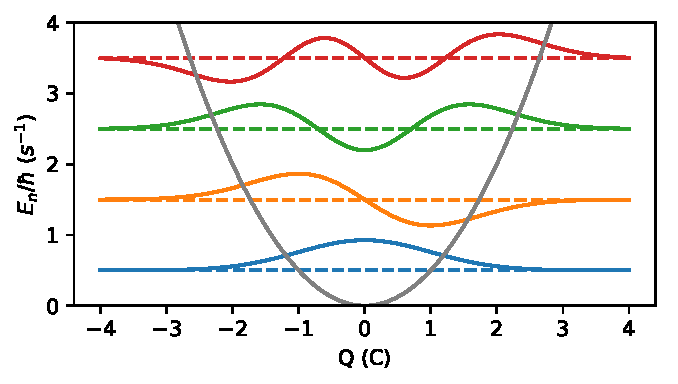
\includegraphics[width=.6\linewidth]{planck_oscillator}
	\caption{Численное решение стационарного уравнения Шредингера для гармонического осциллятора: изображены низшие четыре собственных энергетических уровня (штриховые линии) и состояния гамильтониана (цветные сплошные линии, не в масштабе, за ноль принят соответствующий уровень энергии). Серая сплошная линия показывает потенциальную энергию системы. Параметры $L = 1$ Гн, $ C = 1$ Ф дают циклическую частоту перехода в 1 рад/c.}
	\label{fig:planck_oscillator}
	% построено с помощью Finite difference eigensolver в папке /home/gleb/Projects/Examples/
\end{figure}


Идентичный результат был бы получен при использовании потокового базиса. Однако интересно также рассмотреть энергетический базис, в котором оператор Гамильтона будет диагональным. Для перехода в него будет использоваться так называемое ``вторичное квантование'', использующее операторы рождения и уничтожения фотонов в осцилляторе $\hat a^\dag$ и $\hat a$, $[\hat a, \hat a^\dag] = 1$. Произведением замены 
\begin{align}
	\hat Q \rightarrow \sqrt{\frac{\hbar \omega_r C}{2}}(\hat a^\dag + \hat a),\\
	\hat \Phi \rightarrow i\sqrt{\frac{\hbar \omega_r L}{2}}(\hat a^\dag - \hat a)
\end{align}
гамильтониан приводится к диагональному виду:
\begin{equation}
	\hat{\mathcal H} =  \hbar \omega_r (\hat a^\dag \hat a + 1/2).
\end{equation}

Ненулевая энергия флуктуаций заряда в основном состоянии оказывается проблемой в случае квантования электромагнитного излучения в вакууме: свободное излучение после преобразования Фурье может представляется квантовомеханически как набор квантовых осцилляторов с непрерывным спектром всевозможных частот. Если учесть, что в основном состоянии энергия каждого равна $\hbar \omega/2$, интеграл полной энергии флуктуаций вакуума окажется расходящимся. Даже если взять в интеграле некоторую верхнюю отсечку по частоте, как часто делается в квантовой электродинамике, энергия пустого пространства окажется на 120 порядков больше, чем предсказывается космологической постоянной в общей теории относительности; в то же время, гравитационного эффекта, который был бы вызван энергией нулевых флуктуаций, действительно не наблюдается. С другой стороны, действие вакуумных флуктуаций однозначно проявляется в так называемом эффекте Казимира, измеренном сейчас с большой точностью \cite{zou2013casimir}. Подобно ультрафиолетовой катастрофе конца 19 века, эта проблема названа вакуумной катастрофой и до сих пор не разрешена \cite{adler1995vacuum}.

\subsection{Квантование произвольных электрических цепей по Деворе}

На заре экспериментов с макроскопическими квантовыми системами Мишелем Деворе была создана методика для квантования произвольных электрических цепей, которая отразилась в его методичке 1995 года ``Квантовые флуктуации в электрических цепях'' \cite{devoret1995quantum}. По большому счету, в этой работе не содержится ничего, чего не было бы в стандартных аналитической и квантовой механиках, однако есть несколько практических замечаний, которые пригодятся нам в дальнейшем при рассмотрении более сложных электрических цепей, содержащих джозефсоновсие переходы.

Подход Деворе -- квантовать цепи в потоковом базисе, учитывая возможное наличие петель, через которые может проходить внешний магнитный поток. Такой поток оказывается важен, так как его изменение может создавать ЭДС в замкнутом контуре и явно входить во второй закон Кирхгофа. Если работать в потоковом базисе (проинтегрировать все напряжения во втором законе Кирхгофа по времени), такой поток окажется просто включенным в уравнения, и, следовательно, в Лагранжиан. 

Поучительным в данном случае является пример гармонического осциллятора, который формально представляет собой кольцо, в котором можно записать второй закон Кирхгофа. Представим, что в через данное кольцо физически проходит некий поток $\Phi_e$. Тогда в потоковом базисе второй закон Кирхгофа запишется как
\begin{equation}
	-L\dot I_L - Q_C/C = \dot \Phi_e.
\end{equation}
Интегрируя по времени и подставляя в первый закон Кирхгофа, получим:
\begin{equation}
	\Phi_L/L = - (\ddot \Phi_L + \ddot \Phi_e)C.
\end{equation}
Как можно видеть, в случае электрического осциллятора в уравнение движения входит вторая производная от внешнего потока. Таким образом, если он является постоянным или даже линейно меняющимся во времени, никакого эффекта на динамику он не оказывает. В противном же случае его надо учитывать в явном виде.

Посмотрим теперь, как подходит к этой проблеме Деворе. В формуле (2.13) из \cite{devoret1995quantum} мы обнаруживаем, как второй закон Кирхгофа учитывается при определении потоковой переменной на элементе, заканчивающем неустранимый контур. Такой элемент не создает новой степени свободы в системе, а лишь использует старые степени свободы (узловые потоки, см. определение там же \cite{devoret1995quantum}). Для демонстрации подхода несколько усложним контур электрического осциллятора, добавив в него новую индуктивность параллельно или последовательно со старой, см. \autoref{fig:llc}.
\begin{figure}
	\centering
	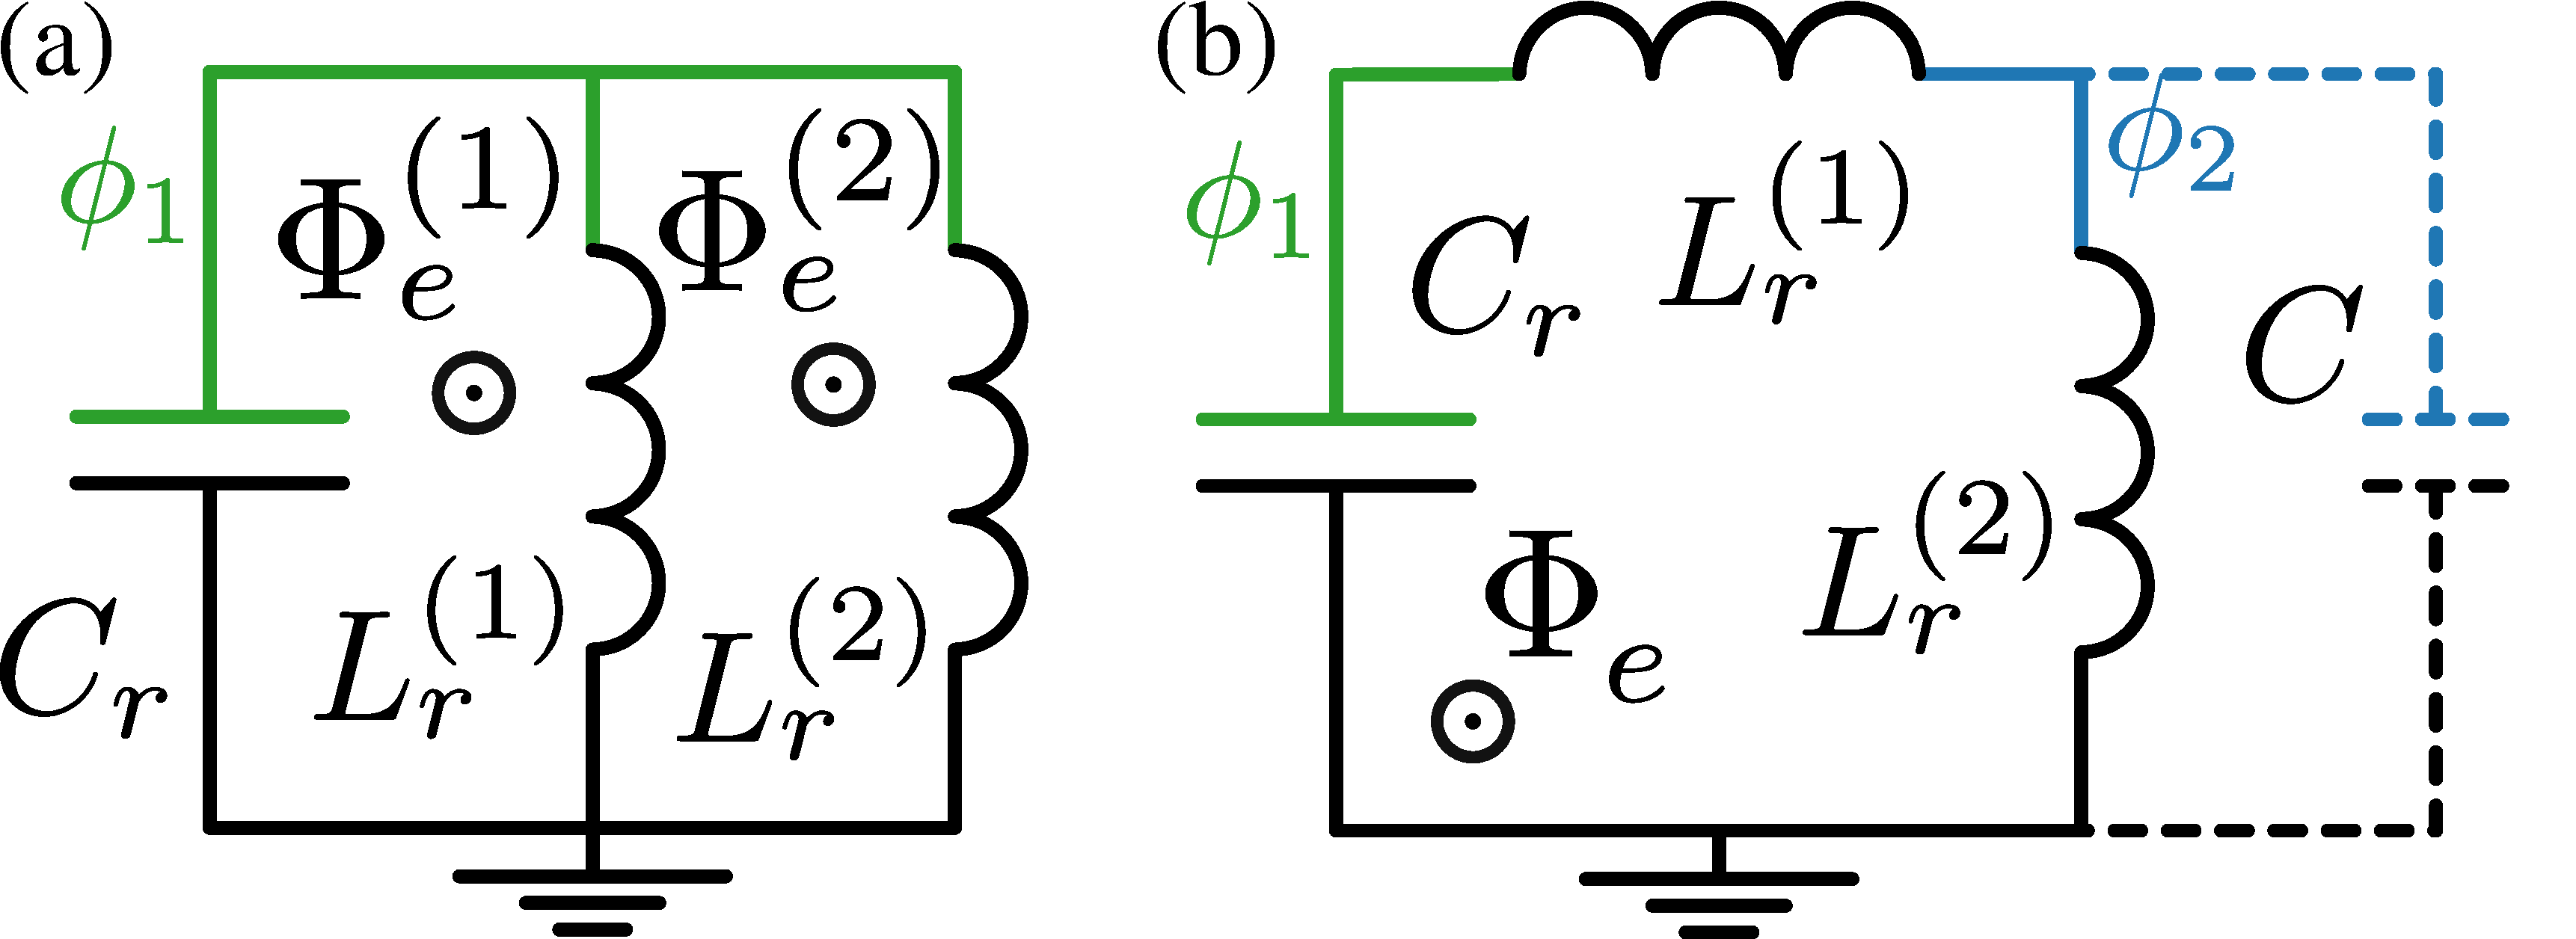
\includegraphics[width=0.8\linewidth]{Pictures/LLC}
	\caption{Две конфигурации осциллятора с добавленными индуктивностями: параллельно \textbf{(a)} и последовательно \textbf{(b)}. Узловые фазовые переменные (степени свободы) обозначены буквами $\phi$ и соответствующим цветом.}
	\label{fig:llc}
\end{figure}

Для параллельного соединения обе индуктивности являются элементами, закрывающими свой контур. Поэтому для катушек мы записываем:
\begin{align}
	\Phi_L^{(1)} &= \phi_1 - 0 + \Phi_e^{(1)},\\
	\Phi_L^{(2)} &= \phi_1 - 0 + \Phi_e^{(2)},
\end{align}
где мы использовали тот факт, что ``земля'' имеет по определению нулевое значение узлового потока. В таком случае лагранжиан в потоковом базисе запишется как 
\begin{equation}
	\mathcal{L}_{L||L||C} = \frac{C_r \dot\phi_1^2}{2} - \frac{\left(\phi_1 + \Phi_e^{(1)}\right)^2}{2L_r^{(1)}} - \frac{\left(\phi_1 + \Phi_e^{(2)}\right)^2}{2 L_r^{(2)}}.
\end{equation}

Как видим, внешние потоки явно входят в лагранжиан, и, очевидно, будут присутствовать и в гамильтониане системы. Однако при ближайшем рассмотрении потенциала выясняется, что его форма остается неизменной параболической для любых конфигураций значений индуктивностей и потоков сквозь петли; единственным эффектом внешних потоков является постоянное смещение минимума потенциальной энергии относительно параметра $\phi_1$. Колебания же будут определяться квадратичным членом с эффективной индуктивностью $L_r = L_r^1 || L_r^2$ параллельно соединенных катушек. Тот же результат мы получили бы, если бы заранее объединили катушки согласно правилу сложения индуктивностей и применяли процедуру к уже упрощенному контуру (предварительное упрощение часто применяется для сложных цепей, см., например, \cite{koch2007charge}). 

Рассмотрим теперь последовательное соединение катушек, \autoref{fig:llc}~(b) (без штрихованного конденсатора). В отличие от предыдущего случая, мы обнаруживаем, что число степеней свободы увеличилось с добавлением новой индуктивности, а единственный контур сохранился. Лагранжиан такой системы:
\begin{equation}
	\mathcal{L}_{LL||C} = \frac{C_r \dot\phi_1^2}{2} - \frac{(\phi_2 - \phi_1)^2}{2L_r^{(1)}} - \frac{\left(\phi_2+\Phi_e\right)^2}{2 L_r^{(2)}}.\label{eq:ll||c}
\end{equation}

Из вида лагранжиана становится очевидно, что переменная $\phi_2$ оказывается зависимой. Действительно, уравнение Лагранжа-Эйлера на нее запишется следующим образом:
\begin{equation}
	\phi_2/L_r^{(1)} + \phi_2/L_r^{(2)} + \Phi_e/2L_r^{(2)} = \phi_1/L_r^{(1)}.
\end{equation}
Подставляя выраженное отсюда $\phi_2$ в оставшееся уравнение Эйлера-Лагранжа, мы получим уравнение колебаний на $\phi_1$ с эффективной индуктивностью $L_r^{(1)} + L_r^{(2)}$. Очевидно, именно так и должно было получиться, если бы мы опять применили правило сложения теперь уже последовательных индуктивностей. Магнитный поток, конечно, также войдет в уравнения движения, но не будет влиять на динамику системы при условии независимости его от времени. 

Но каковы же будут решения уравнения Шредингера, составленного с использованием лагранжиана \eqref{eq:ll||c}? Из-за отсутствия обобщенного импульса по $\phi_2$ ($\partial \mathcal{L}_{LL||C}/\partial \dot \phi_2 = 0$) в операторе Гамильтона не будет второй производной по этой координате. Это приведет к тому, что собственные функции в направлении $\phi_2$ окажутся дельта-функциями и суперпозициями дельта-функций. Также это будет означать, что в силу соотношения неопределенностей узловой заряд $q_2$ на острове, отмеченном синим на \autoref{fig:llc}~(b), окажется полностью делокализованным, так как является канонически сопряженным бесконечно локализованному дельта-функцией узловому потоку $\phi_2$. Численное решение такого уравнения Шрёдингера оказывается невозможным, так как спектр задачи является непрерывным и не может быть воспроизведен диагонализацией конечномерных матриц. Результаты такого наивного решения приведены на \autoref{fig:llcstatesdelta}~(a). Как можно видеть, алгоритм воспроизводит дискретные дельта-функции по оси $\phi_2$ и правильно определяет структуру собственного состояния гармонического осциллятора по оси $\phi_1$, однако рассчитанный энергетический спектр системы оказывается в целом неверным. Физически полная делокализация узлового заряда также невозможна, так как означала бы ненулевую вероятность обнаружения произвольно большого заряда на соответствующем острове. 

\begin{figure}
	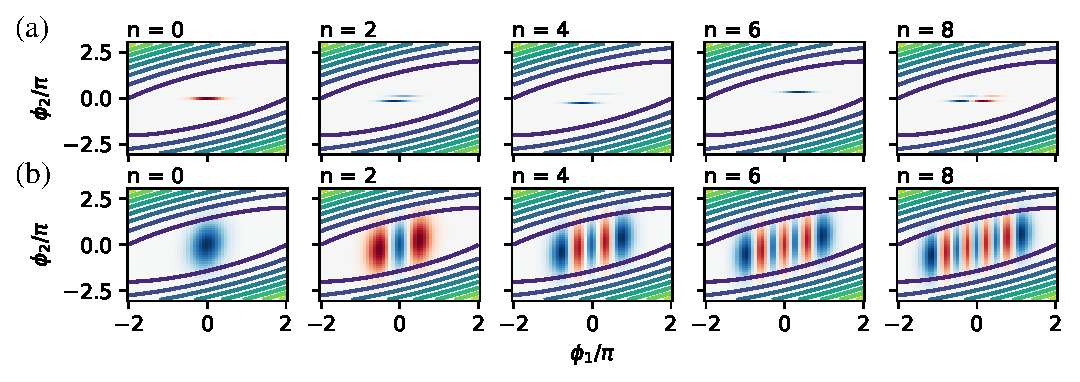
\includegraphics[width=\linewidth]{Pictures/llc_states}
	\caption{Собственные состояния модели \autoref{fig:llc}~(b) при $C = 0$ \textbf{(a)} и $C = C_r/100$ \textbf{(b)} (показаны чётные номера). В обоих случаях $C_r = 1, L_r^{(1)} = L_r^{(2)} = 0.5$. При $C = 0$ численные собственные значения зависят от шага сетки и оказываются неверными. В другом случае же ответ получается верным: спектр эквидистантный с шагом $\omega_r \approx 1\ \text{s}^{-1}$. Контурными линиями показана потенциальная энергия из \eqref{eq:ll||c}. В каждом направлении пространство разбито на 50 ячеек.}
	\label{fig:llcstatesdelta}
	% построено с помощью Finite difference eigensolver в папке /home/gleb/Projects/Examples/
\end{figure}

Как видим, в классическом случае схема \autoref{fig:llc}~(b) без штрихованного конденсатора допускает физически осмысленное решение. Однако в квантовом случае для получения осмысленного результата требуется учитывать малый конденсатор $C$ для освобождения потоковой переменной $\phi_2$ (для простоты будем считать, что в новом кольце поток равен нулю). На практике такая емкость всегда будет существовать из-за конечных размеров проводника, отмеченного синим цветом. Интересно также, что переход от локализации к делокализации $\phi_2$ происходит скачком при непрерывном уменьшении емкости конденсатора до нуля. Пример состояний, получающихся при правильной диагонализации изображен на \autoref{fig:llcstatesdelta}~(b). Как видим, структура волновой функции в направлении $\phi_2$ предполагает основное состояние нового дополнительного осциллятора. 

Для полноты картины требуется также определить, какая структура колебаний будет у классической модели с дополнительным конденсатором. При добавлении новой степени свободы для нахождения нормальных мод колебаний потребуется решить вековое уравнение:
\begin{equation}
	\text{det}(\Pi - \lambda T) = 0,
\end{equation}
где $T$ -- квадратичная форма потенциальной энергии, а $\Pi$ -- квадратичная форма кинетической энергии системы. Лагранжиан с учётом добавленной емкости:
\begin{equation}
\mathcal{L}_{LL||C+C} = \frac{C_r \dot\phi_1^2}{2} + \frac{C \dot\phi_2^2}{2} - \frac{(\phi_2 - \phi_1)^2}{2L_r^{(1)}} - \frac{\phi_2^2}{2 L_r^{(2)}}.
\end{equation}
Используя модифицированный лагранжиан, получаем следующие выражения:
\begin{equation}
	\Pi = \left(
	\begin{matrix}
	\frac{1}{L_r^{(1)}}&-\frac{1}{L_r^{(1)}}\\
	-\frac{1}{L_r^{(1)}}&\frac{L_r^{(1)}+L_r^{(2)}}{L_r^{(1)}L_r^{(2)}}
	\end{matrix}\right),\ 
	T = \left(
	\begin{matrix}
	C_r& 0 \\
	0 & C
	\end{matrix}\right).
\end{equation}
Разложение в ряд Тейлора решений векового уравнения вблизи $C = 0$ дает два решения:
\begin{equation}
	\lambda_{1,2} = \frac{1}{C_r\left(L_r^{(1)}+L_r^{(2)}\right)},\quad \frac{L_r^{(1)}+L_r^{(2)}}{C L_r^{(1)}L_r^{(2)}}.
\end{equation}
Видно, что колебания дополнительного осциллятора в случае малой емкости его острова происходят на очень высокой частоте $\sqrt{\lambda_2}$. На языке импедансов можно сказать, что реактивное сопротивление большого конденсатора $C_r$ в этом режиме стремится к нулю, и он может быть заменен закороткой. Тогда сразу становится понятна и форма ответа для частоты колебаний побочного осциллятора: эффективная индуктивность складывается из параллельно подключенных $L_r^{(1)}$ и $L_r^{(2)}$. Таким образом, мы определили, как корректно работать с последовательно подключаемыми индуктивностями и в квантовом случае, и в классическом.

\begin{figure}
	\centering
	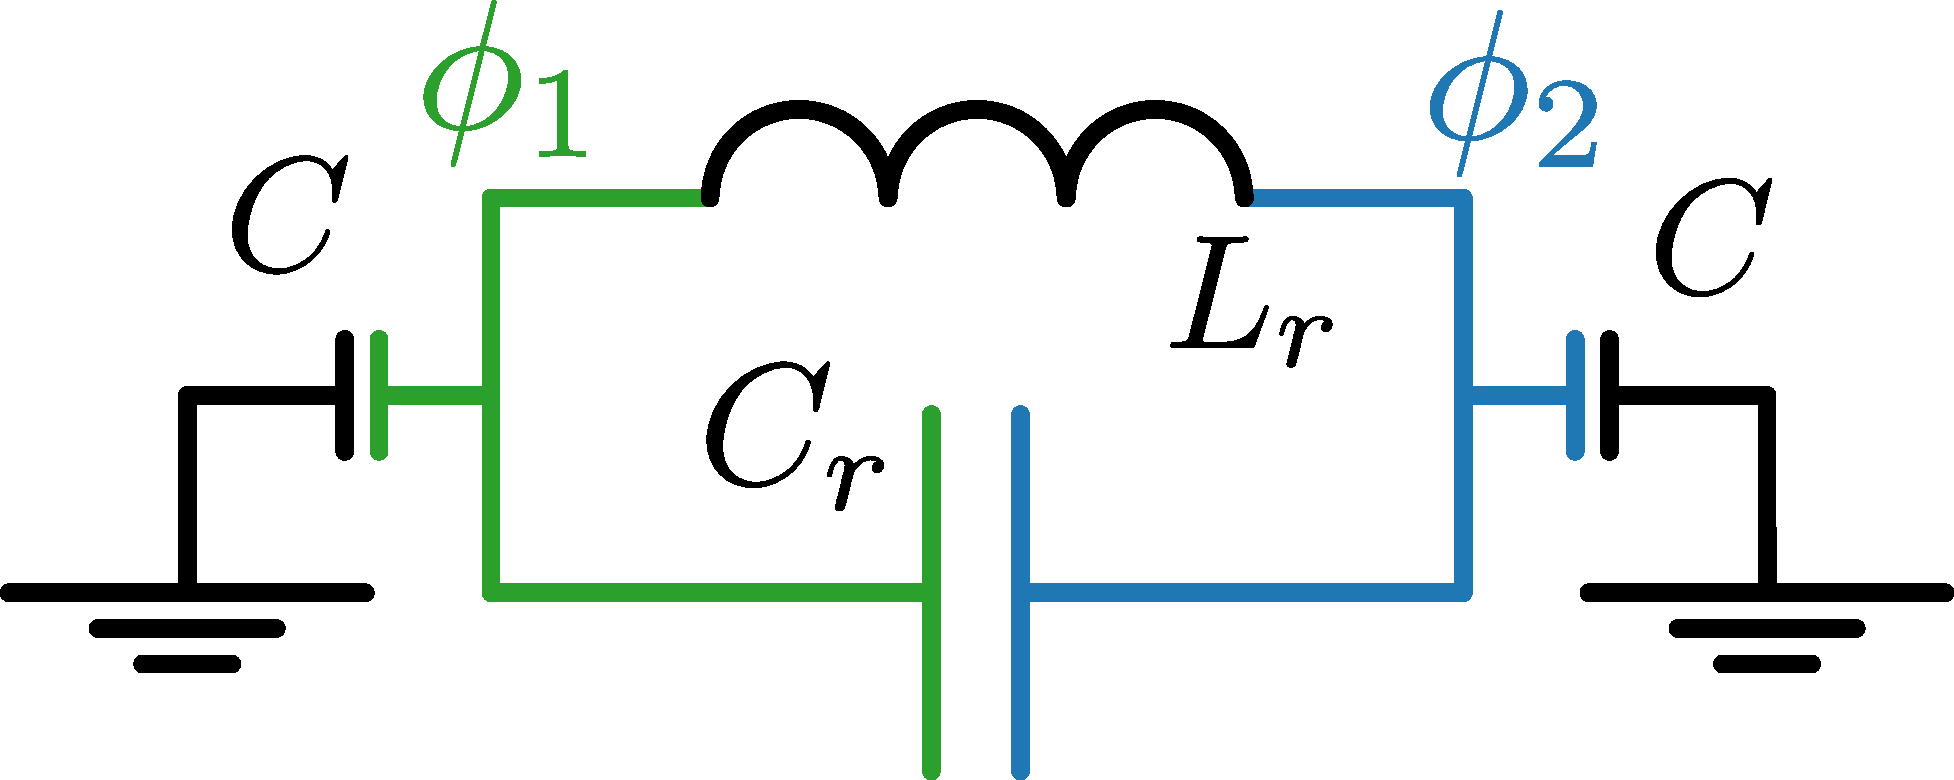
\includegraphics[width=0.5\linewidth]{Pictures/lc_cap_inv}
	\caption{Осциллятор, заземленный через конденсаторы малой ёмкости.}
	\label{fig:lccapinv}
\end{figure}

Добавление малых емкостей на землю параллельно уже существующим большим конденсаторам может привести к подобным проблемам в случае решения задач в зарядовом базисе. Рассмотрим пример такой проблемы для еще одной электрической схемы, изображенной на \autoref{fig:lccapinv}. Лагранжиан системы запишется как
\begin{equation}
	\mathcal{L}_{LCg} = \frac{C \dot \phi_1^2}{2} + \frac{C \dot \phi_2^2}{2} + \frac{C_r\left(\dot\phi_1 - \dot\phi_2\right)^2}{2} - \frac{L_r \left(\phi_1  - \phi_2\right)^2}{2}.\label{eq:l_lcg}
\end{equation}
Как видим, квадратичная форма кинетической энергии (коэффициенты её также называются матрицей ёмкостей) здесь не приведена к диагональному виду. Поэтому чтобы получить гамильтониан через преобразование Лежандра, потребуется решить систему линейных уравнений на $\phi_{1,2}$ относительно $q_{1,2}$. После этого гамильтониан запишется как 
\begin{equation}
	\mathcal{H}_{LCg} = \frac{1}{2} \left(\begin{matrix} q_1\\q_2\end{matrix}\right) \left(\begin{matrix}
	C+C_r & -C_r \\
	-C_r & C+C_r
	\end{matrix}\right)^{-1}\left(\begin{matrix} q_1&q_2\end{matrix}\right)+\frac{L_r \left(\phi_1  - \phi_2\right)^2}{2}.
\end{equation}
Проблема здесь заключается главным образом в том, что потенциальная энергия не имеет роста по направлению $\phi_1 + \phi_2$, и волновые функции окажутся делокализованными. Очевидно, что такая проблема не возникла бы, если бы мы изначально исключили энергии малых конденсаторов из лагранжиана и осуществили бы замену координат $\phi_1 - \phi_2 \rightarrow \phi$, уменьшив реальное число степеней свободы. Проанализируем, насколько эта ситуация сходна с предыдущей.

Для начала попробуем решить вековое уравнение, задаваемое \eqref{eq:l_lcg}. Его решениями окажутся
\begin{equation}
	\lambda_{1,2} = 0,\ \frac {1}{L_r \left( C/2 + C_r \right) }.	
\end{equation}
Нулевое решение сразу говорит нам о том, что система может существовать в состоянии безразличного равновесия когда $\phi_1 = \phi_2$. Физически это означает, что потенциалы на островах равны во все моменты времени, а заряды их, соответственно, должны быть какими угодно, но одинаковыми. Ненулевое решение отвечает осцилляциям, в которых малые конденсаторы складываются последовательно друг с другом, а затем параллельно с конденсатором $C_r$. Выражение легко понять, если вместо соединения конденсаторов $C$ землей соединить их друг с другом, а землю вообще исключить из схемы. В целом мы видим, что классическое решение, основанное на вековом уравнении, не встречает трудностей с такой системой.

Решение уравнения Шрёдингера численно методом конечных разностей в такой постановке невозможно. Частица в заданном потенциале будет иметь непрерывный энергетический спектр, для которого, как уже обсуждалось ранее, дискретизовать задачу в принципе нельзя. Поэтому для успешного численного решения в подобных ситуациях требуется сначала провести аналитическую замену координат:
\begin{equation}
	\begin{aligned}
		\phi_1 &= \frac{\phi_+ + \phi_-}{2},\\
		\phi_2 &= \frac{\phi_+ - \phi_-}{2}.
	\end{aligned}
\end{equation}
Тогда лагранжиан запишется в виде
\begin{equation}
	\mathcal{L}_{LCg} = \frac{(C_r+C/2)\dot\phi_-^2}{2}  + \frac{C \dot\phi_+^2}{4} - \frac{L_r \phi_-^2}{2}.
\end{equation}
Фактически, был произведен переход к нормальным координатам, и уравнения на степени свободы разделились. Нахождение обратной матрицы емкости теперь не представляет трудности, и гамильтониан запишется как 
\begin{equation}
	\mathcal{H}_{LCg} = \frac{q_-^2}{2(C_r+C/2)} + \frac{q_+^2}{C} + \frac{L_r \phi_-^2}{2}.
\end{equation}
Переходя к операторному виду, будем искать решения уравнения Шрёдингера в виде $\psi(\phi_+, \phi_-) = \psi_+(\phi_+)\psi_-(\phi_-)$, a общую энергию в виде $E = E_1+E_2$. После разделения переменных по методу Фурье, получим два уравнения
\begin{equation}
	\begin{aligned}
	-\frac{\hbar^2}{C}\frac{\partial^2}{\partial \phi_+^2}\psi_+ - E_1\psi_+ &= - \lambda\psi_+,\\
	-\frac{\hbar^2}{2(C_r + C/2)}\frac{\partial^2}{\partial \phi_-^2}\psi_- + \frac{L_r \phi_+^2}{2}\psi_- - E_2\psi_+ &= \lambda\psi_-.
	\end{aligned}
\end{equation}
Обозначая собственные энергии как $E^+ = E_1 - \lambda,\ E_n^- = E_2 + \lambda$, получим для исходных энергий $E = E^+ + E_n^-$. Первое уравнение решается аналитически и дает непрерывный спектр, второе же воспроизводит задачу для одномерного гармонического осциллятора с эффективной емкостью $C_r+C/2$. Таким образом, после замены разделения переменных решение задачи численно становится возможным. 

В заключение, обозначим дуализм между двумя проблемными случаями, описанными выше. В первом случае дополнительная степень свободы не давала вклад в кинетическую энергию системы, а во втором случае -- в потенциальную. С учетом того, что роль кинетической и потенциальной энергии выбирается при выборе обобщенных координаты и импульса, разницы между двумя этими ситуациями на самом деле нет. В обоих случаях проблемы с численным решением были вызваны непрерывностью спектра системы. Однако в первом случае, в отличие от второго, нельзя разделить переменные в уравнения Шрёдингера и получить аналитическое решение для степени свободы с непрерывным спектром. Поэтому для успешного численного решения необходимо ввести дополнительный элемент, локализующий заряд на острове. Точно также можно было бы ввести большие по величине индуктивности во втором примере параллельно с малыми конденсаторами для локализации узлового потока. Локализация и делокализация связаны с известным свойством преобразования Фурье:
\begin{equation}
	2\pi\, \delta(\phi) = \int\limits_{-\infty}^{\infty} e^{iq\phi} \diff q,
\end{equation}
и тем фактом, что волновые функции в представлениях канонически сопряженных переменных являются Фурье-образами друг друга. В дальнейшем мы еще затронем тему квантования сверхпроводниковых цепей, так как джозефсоновские переходы вносят в неё свою специфику, связанную с дискретностью узловых зарядов.


\section{Сверхпроводимость и эффект Джозефсона}

\subsection{Теория Лондонов}

Сверхпроводимость была экспериментально обнаружена в 1911 году голландским ученым Хейке Камерлинг-Оннесом в ртути при гелиевых температурах. Именно он также впервые получил и жидкий гелий, без которого невозможно было бы получить необходимую низкую температуру, за что уже через два года был удостоен Нобелевской премии. Открытие это было скорее случайным, так как никто до этого даже и представить не мог возможность такого эффекта, не то что предсказать его. Впоследствии достаточно долго считалось, что явление заключается лишь в падении до нуля электрического сопротивления металлов, и только в 1933 году немцами Вальтером Мейсснером и Робертом Оксенфельдом был обнаружен эффект абсолютного диамагнетизма сверхпроводников. 

Первым шагом к пониманию природы сверхпроводимости стала феноменологическая теория немецких физиков Фрица и Хайнца Лондонов \cite{london1935electromagnetic}. Рассуждение авторов начинается с ``уравнения ускорения'', которое было принято в то время для описания ``сверхпроводящих'' электронов, движущихся без трения:
\begin{equation}
	\Lambda \dot{\mathbf{J}} = \mathbf{E},\ \Lambda = m/ne^2. \label{eq:acceleration}
\end{equation}
Здесь $m$ -- это масса сверхпроводящих электронов, $e$ -- их заряд, $n$ -- концентрация. Если взять ротор от этого уравнения, учесть третье уравнение Максвелла и тот факт, что дивергенция магнитного поля равна нулю, а затем проинтегрировать по времени, то можно получить следующее равенство:
\begin{equation}
	\Lambda c^2 \nabla^2 (\mathbf{H}-\mathbf{H}_0) = \mathbf{H} - \mathbf{H}_0,\label{eq:london_inhomogeneous}
\end{equation}
где $\mathbf{H_0}$ -- это значение напряжённости магнитного поля в некий нулевой момент времени. Физически осмысленные решения однородного уравнения при $\mathbf{H_0} = 0$ оказываются экспоненциально спадающими при углублении в толщу сверхпроводника, а частное решение $\mathbf{H} = \mathbf{H}_0$ таким образом предсказывает возможность ``вмораживания'' начального магнитного поля в сверхпроводник после перехода его в сверхпроводящее состояние. Однако эксперимент Мейсснера опровергает подобный вывод: достаточно слабое магнитное поле выталкивается из сверхпроводника при переходе через критическую температуру. Это и отличает гипотетический идеальный проводник, описываемый уравнением \eqref{eq:acceleration}, от реальных сверхпроводников.

Так как уравнение \eqref{eq:london_inhomogeneous} правильно описывает затухающее внутри сверхпроводника магнитное поле в однородном случае, Лондоны предложили постулировать $\mathbf{H_0} = 0$ и преобразовать однородное уравнение обратно к виду
\begin{equation}
	\nabla \times \Lambda \mathbf J = -\frac{1}{c} \mathbf{H},\label{eq:london_first}
\end{equation}
фактически опуская дифференцирование по времени и константу интегрирования, возникавшую в прямом преобразовании. Данное уравнение уже не приводит к уравнению \eqref{eq:acceleration}. Вместо него может быть получено более слабое утверждение
\begin{equation}
	\nabla \times (\Lambda \dot{\mathbf J} - \mathbf E)  = 0,
\end{equation}
или, что то же самое,
\begin{equation}
	 \Lambda \dot{\mathbf J} - \mathbf E = \nabla \mu. \label{eq:london_second}
\end{equation}
Для соблюдения Лоренц-инвариантности можно выбрать $\mu = -\Lambda c^2 \rho$, $\rho = \nabla\cdot\mathbf E$, и тогда выводится еще одно уравнение:
\begin{equation}
	\Lambda (\dot{\mathbf J} + c^2 \nabla \rho) = \mathbf E.
\end{equation}
Отсюда следует, что 
\begin{gather}
	\Lambda c^2 \nabla^2 \mathbf E = \mathbf E,\\
	\Lambda c^2 \nabla^2 \rho = \rho.
\end{gather}
Такие уравнения предполагают, что статическое электрическое поле проникает в сверхпроводник так же, как и статическое магнитное, экспоненциально затухая на глубине $d = \sqrt{\Lambda c^2}$. Однако, как вскоре выяснилось, такой выбор $\mu$ для соблюдения Лоренц-инвариантности является неверным. Чтобы проверить, действительно ли электрическое поле проникает внутрь сверхпроводника, через несколько месяцев после вышеописанной работы Хайнц Лондон провел эксперимент с ртутным конденсатором \cite{london1936experimental}. В случае, если проникновение поля в сверхпроводящей фазе имело бы место, то емкость такого конденсатора при сверхпроводящем переходе уменьшилась бы на величину порядка $2d$ из-за эффективного удаления обкладок друг от друга. Однако такого эффекта с большой точностью в эксперименте обнаружено не было. Таким образом, статическое электрическое поле в сверхпроводнике существовать не может так же, как и в нормальном металле\footnote{Интересно отметить, что и до сей поры в авторитетных изданиях продолжают выходить публикации, спорящие с этим. Они утверждают, что статическое электрическое поле в сверхпроводник всё-таки проникает, причем на основе этого эффекта можно даже создать полевой транзистор \cite{de2018metallic, paolucci2018ultra}. Альтернативное объяснение наблюдаемым в указанных работах эффектам можно найти в работе \cite{golokolenov2020origin}.}. Поэтому  правильным выбором калибровки будет $\mu=0$, что возвращает нас к исходному уравнению ускорения \eqref{eq:acceleration}. Подводя итог, запишем правильные уравнения Лондонов современном виде как
\begin{align}
\Lambda c\, \nabla \times \mathbf J &= - \mathbf H,\\
\Lambda \dot{\mathbf J} &= \mathbf E.
\end{align}

\subsection{Теория Пиппарда}

В последующие годы эксперименты со статическим магнитными и электрическими полями в рамках исследования свойств сверхпроводников перетекли к опытам с переменным током. По аналогии с аномальным скин-эффектом в чистых металлах, где длина свободного пробега электронов оказывается сравнима с толщиной скин-слоя, в 1953 году англичанин Брайан Пиппард предложил обобщение эмпирических уравнений Лондонов нелокальным интегральным уравнением \cite{pippard1953experimental}. Исток этой идеи заключается в эксперименте, проведенным автором в той же работе: исследовалась глубина проникновения магнитного поля в олово в зависимости от концентрации примеси индия\footnote{Глубина проникновения измерялась косвенно по изменению частоты сверхпроводящего резонатора при превышении критического магнитного поля \cite{pippard1950surface}.}. Оказалось, что при изменении концентрации индия от 0  до 3\% глубина проникновения магнитного поля менялась практически в два раза, хотя критические температура и магнитное поле менялись несущественно. В то же время, сопротивление загрязненного олова оказывается в 1200 раз выше, а длина свободного пробега в нем электронов во столько же раз ниже. Таким образом, Пиппардом была открыта некая пока необъяснимая связь между длиной свободного пробега электронов в нормальном состоянии и глубиной проникновения магнитного поля в сверхпроводник.

К нелокальному уравнению автор пришел, преобразуя сперва \eqref{eq:london_first} к виду 
\begin{equation}
	\Lambda \mathbf J + \mathbf A = 0,
\end{equation}
где $\mathbf A$ -- это векторный потенциал с правильной калибровкой. Далее Пиппард вводит некую длину $\xi$ в сверхпроводнике по аналогии с длиной свободного пробега, которая фигурирует в законе, напоминающем закон Ома для обычных проводников:
\begin{equation}
	\mathbf J = - \frac{\xi}{\xi_0 \Lambda} \mathbf A.
\end{equation}
Далее постулируется интегральное уравнение:
\begin{equation}
	\mathbf J = - \frac{3}{4\pi \xi_0 \Lambda} \int \mathbf r \frac{ \mathbf r\cdot \mathbf A\, e^{-r/\xi}}{r^4} \diff^3 r.
\end{equation}
Из этого уравнения Пиппардом было получено аналитическое выражение для глубины проникновения (см. формулу (12) из \cite{pippard1953experimental}) в зависимости от введенной постоянной $\xi$. Оказалось, что глубина проникновения в случае $\xi \ll \lambda$ ведет себя как $1/\sqrt{\xi}$, а в противном случае не зависит от $\xi$. Хорошее совпадение с экспериментальными данными дает выражение, связывающее $\xi$ с длиной свободного пробега простым законом пропорциональности (коэффициент определялся в статье методом аппроксимации), однако получить правильное значение для $\xi_0$ -- предела $\xi$ для чистого олова при нулевой температуре -- из такого закона Пиппарду не удалось.

\subsection{Теория БКШ}

Спустя всего 4 года после работы Пиппарда вышла статья американцев Джона Бардина, Леона Купера и Джона Шриффера \cite{bardeen1957theory}, удостоенная впоследствии Нобелевской премии 1972 года, которая построила полностью квантовомеханическую модель для так называемых обычных сверхпроводников. Конечно, эта теория родилась не на пустом месте и была в значительное мере предопределена развитием квантовой теории металлов. Еще в 1937 году Слэтер \cite{slater1937nature} размышлял о природе сверхпроводящего состояния в одноименной работе и предполагал, что теория возмущений, примененная к стандартным блоховским функциям электронов, может породить некоторое ``особенное состояние'', отделенное от основного непрерывного спектра частично заполненной зоны проводника. Отделение приведет к тому, что локальная плотность состояний, видимая электроном, уменьшится практически до нуля, что в стандартной блоховской теории означает отсутствие сопротивления вследствие малой вероятности рассеяния. Помимо этого в 1938 году независимо Петром Капицей \cite{kapitza1938viscosity} (турбулентный случай) и Джоном Алленом и Доном Мизенером \cite{allen1938flow} (ламинарный случай) была окончательно установлена сверхтекучесть гелия-4, а Фриц Лондон предположил, что явление объясняется Бозе-Эйнштейновской конденсацией \cite{london1938lambda}. Явления сверхтекучести и сверхпроводимости были очевидно связаны друг с другом и требовали общего объяснения.

Предвестниками работы БКШ были и достаточно лаконичная работа Бардина \cite{bardeen1955theory}, посвященная вопросу достаточности наличия энергетической щели для объяснения диамагнетизма сверхпроводников, и работа Купера касательно теоретического обоснования существовании энергетической щели в Ферми-газе при введении сколь угодно малого взаимодействия между электронами \cite{cooper1956bound}. Однако, наверное, важнейшим экспериментальным открытием, подтолкнувшего научное сообщество к подробной разработке идеи об электрон-фононном взаимодействии, стал изотоп-эффект \cite{maxwell1950isotope,reynolds1950superconductivity,de1954isotope}, обнаруженный в 1950 году. Оказалось, что различные изотопы ртути имеют разные температуры сверхпроводящего перехода, причем чем меньше масса ядер, тем больше критическая температура. Как раз тогда же, в начале 1950-х годов, Бардин и Герберт Фрёлих практически одновременно друг с другом развивали теорию взаимодействия электронной и фононной подсистем; описание двух теорий можно найти в работе \cite{bardeen1951electron} (стоит отметить, что Фрёлих также пытался объяснить сверхтекучесть в конце 30-х годов). Однако первоначальный подход, опиравшийся главным образом на идею модификации собственных энергий электронов, встретился с трудностями, которые не позволяли назвать эти теории успешными \cite{bardeen1957theory}. Только после точного описания электрон-фононного взаимодействия с учетом электрического экранирования \cite{bardeen1955electron} удалось построить действительно непротиворечивую модель сверхпроводимости, которая используется и по сей день.

В данной работе мы будем пользоваться лишь основными выводами из теории БКШ: наличие общей волновой функции основного состояния куперовских пар с фазой $\phi$. Если фаза зависит от трехмерных координат, то наблюдается течение сверхтока. В этом контексте также можно упомянуть и феноменологическую теорию Льва Ландау и Виталия Гинзбурга, созданную в начале 1950-х годов. Коэффициенты теории вычисляются из теории БКШ \cite{gor1959microscopic}.

\subsection{Эффект Джозефсона}

В 1962 году британский физик Брайан Джозефсон опубликовал работу, предсказывающую два необычных эффекта в связанных сверхпроводниках: первый эффект заключается в том, что при достаточно малом расстоянии между сверхпроводниками через зазор может течь сверхток, а при конечном напряжении на зазоре кроме постоянного сверхтока должен протекать еще и переменный сверхток с частотой, пропорциональной этому напряжению \cite{josephson1962possible}. Вывод в оригинальной работе не слишком изощрен и базируется на модельном гамильтониане
\begin{equation}
	H = \sum_k n_k E_k + \mu_l N_l + \mu_r N_r + \sum_{l,r} T_{lr}a^\dag_l a_r + T_{rl} a^\dag_r a_l, \label{eq:josephson_tunnel}
\end{equation}
где $n_k$ -- число квазичастиц в сверхпроводниках, $\mu_{l,r}$ -- химические потенциалы, определяемые электрическими напряжениями на них $N_{r,l}$ -- числа электронов справа и слева от барьера. Последняя же часть описывает предполагаемое туннелирование электронов со скоростями $T_{lr}$. 

Исторически этот подход опирается на экспериментальные статьи, исследовавшие туннелирование электронов сквозь тонкие диэлектрические барьеры, разделяющие электроды из нормального металла. Например, в работе Дж. К. Фишера и Айвара Джайевера 1960 года  \cite{fisher1961tunneling} измерялось сопротивление тонких оксидных барьеров на алюминии при комнатной температуре. Толщина барьера измерялась по величине электрической емкости между электродами принимая $\epsilon_{Al_2O_3} = 8$. Экспоненциальная зависимость тока от напряжения позволила установить факт туннелирования сквозь барьер при небольших напряжениях порядка 1 В (теоретическая модель туннелирования еще в 1951 году была построена Рагнаром Холмом \cite{holm1951electric}). За год до этого Джайевером измерялись и вольт-амперные характеристики переходов сверхпроводник-изолятор-сверхпроводник \cite{giaever1960energy, giaever1960electron}, однако сверхтока он не обнаружил из-за недостаточной фильтрации сигналов. Еще раньше, начиная с 1958 года, Ганс Мейсснер исследовал сопротивление контактов металл-сверхпроводник \cite{meissner1958measurements, meissner1960superconductivity}, которое уменьшалось до нуля при достаточно малых толщинах нормального электрода. Это позволило сделать вывод о том, что плотность ``сверхпроводящих'' электронов падает в металлическом барьере плавно, а не исчезает сразу же, а значит, возможно и их квантовое туннелирование.

Непосредственно предшествующей статье Джозефсона была работа Моррела Кохена, Леопольдо Фаликова и Джеймса Филлипса 1962 года \cite{cohen1962superconductive}, в которой использовался точно такой же туннельный Гамильтониан. В своей статье авторы пытались построить математическую модель, которая бы описывала вольт-амперные характеристики переходов нормальный металл-барьер-сверхпроводник. Изначально предполагалось также описать и случай контакта сверхпроводник-барьер-сверхпроводник, однако эта часть работы опубликована не была. 

Интересно, что Джон Бардин с осторожностью относился и к результатам Кохена, и к выводу Джозефсона. В частности, он не спешил признавать, что куперовские пары могут хоть сколько-нибудь проникать в изолирующий барьер \cite{josephsonnobel}. В работе \cite{bardeen1961tunnelling}, посвященной теоретическому обоснованию экспериментальных результатов по туннельным контактам, он отмечает, что энергетическая щель в барьере исчезает практически мгновенно, а значит спаривания электронов там быть не может. Соответственно, в такой ситуации невозможно и туннелирование пар.

С другой стороны, теоретическое научное сообщество постепенно осознавало, что эффекты Джозефсона всё же могут иметь место. Например, в 1963 году к такому выводу пришли Винай Амбегаокар и Алексис Баратофф, после того, как применили теорию Льва Горькова к гамильтониану \eqref{eq:josephson_tunnel} \cite{ambegaokar1963tunneling}. В своей статье они ссылаются на весьма примечательную работу Ричарда Прэнджа \cite{prange1963tunneling}, которая будет опубликована в том же году с точно таким же названием, как у упомянутой ранее статье Бардина, отмечавшей невозможность спаривания электронов в барьере. Прэндж обосновал использование туннельного гамильтониана в форме \eqref{eq:josephson_tunnel} и также высказывался в поддержку расчета Джозефсона.

Амбегаокару и Баратову удалось вывести строгое выражение для изменения числа частиц на одном из островов:
\begin{equation}
	I = e \langle \dot N_l \rangle =  \frac{i}{\hbar}\langle [H, N_l] \rangle = I_c \sin(\alpha + \alpha'),
\end{equation}
где $\alpha'$ -- это вспомогательный угол, аргумент комплексных чисел, использовавшихся в расчете, смысл $\alpha$ будет раскрыт ниже, а 
\begin{equation}
	I_c = \frac{\Delta_1(T)}{R_n} K \left(\sqrt{1 - \Delta_1^2(T)/\Delta_2^2(T)}\right),
\end{equation}
где $\Delta_{1,2}(T),\ \Delta_1(T) < \Delta_2(T)$ -- величины энергетических щелей в сверхпроводниках, между которыми наблюдается эффект, в зависимости от температуры $T$, $K(x)$ -- полный эллиптический интеграл первого рода ($K(0) = \pi/2$), $R_n$ -- сопротивление перехода в нормальном состоянии.

В своей работе Амбегаокар и Баратов не касались вопроса о нестационарном эффекте Джозефсона при конечном напряжении. Однако они ссылаются на еще одну весьма интересную работу Прэнджа и Феррелла, в которой можно найти элегантный вывод обоих эффектов Джозефсона \cite{ferrell1963self}. Проводя аналогию с электроном в периодическом потенциале кристаллической решетки, авторы указывают на то, что при равенстве химических потенциалов на берегах перехода для перенесения $\nu$ пар электронов с одного сверхпроводника на другой не требуется энергия. Поэтому собственные состояния образуются блоховскими суперпозицями вида
\begin{equation}
	\Psi_\alpha = \sum_\nu e^{i\alpha \nu} \Psi_\nu,
\end{equation}
где $\hbar\alpha$ -- ``квазиимпульс'', переменная, сопряженная канонически протуннелировавшему числу пар. Форма энергетической зоны опишется уравнением
\begin{equation}
	E(\alpha) = -\frac{1}{2}\hbar J_1 \cos \alpha,
\end{equation} 
где $\hbar J_1$ -- это умноженный на 4 недиагональный элемент гамильтонина, связывающий состояния $\nu$ и $\nu+1$. Далее, если считать, что таким образом мы записали кинетическую часть гамильтониана, то уравнения движения с линейной потенциальной энергией $U(t) = 2eV(t)\nu$ запишутся согласно теореме Эренфеста как 
\begin{align}
	\frac{\diff \langle \nu \rangle }{\diff t} &=\left\langle \frac{\partial E(\alpha)}{ \partial \hbar\alpha}\right\rangle = \frac{1}{2} J_1 \langle \sin \alpha \rangle,\\
	\frac{\diff \hbar\langle  \alpha \rangle}{\diff t} &= 2 e V(t).\label{eq:JJ2}
\end{align}
Следует отметить, что перенос среднего значения в правой части первого уравнения на аргумент представляет собой достаточно тонкую операцию, и в статье она выполнена с оговорками. Однако несмотря на это, именно такая формулировка хорошо проясняет не только смысл $\alpha$ в статье Амбегаокара и Баратова (на столько меняется фаза комплексного состояния конденсата при туннелировании пары), но и физические корни обоих уравнений Джозефсона в целом. Далее в тексте мы будем использовать обозначение $\varphi$ для разности фаз между берегами джозефсоновского перехода.

Венцом исследований стала экспериментально подтвердившая эффект работа 1963 года \cite{anderson1963probable}, в которой Филип Андерсон и Джон Роувелл, предположив, что температурные шумы измерительной схемы могут подавлять сверхпроводимость, изготовили несколько образцов с более низким, чем обычно, нормальным сопротивлением, чтобы сократить возможное тепловыделение в нормальном состоянии. Доказательством природы наблюдаемого эффекта в первую очередь была найденная характерная зависимость от магнитного поля, подаваемого на образец.

Для параллельно соединенных джозефсоновских переходов с критическими токами $I_{c1}$ и $I_{c2}$ можно классическим образом записать следующий закон зависимости тока от разностей фаз на них:
\begin{equation}
	I = I_{c1}\sin \varphi_1 + I_{c2}\sin \varphi_2 = I_{c\Sigma} \cos \varphi_- \sqrt{1+d^2 \tg^2 \varphi_-} \sin (\varphi_+ + \phi_0),
\end{equation}
где $\varphi_{\pm} = (\varphi_1 \pm \varphi_2)/2$, $\tan \phi_0 = d \tan \varphi_-$. Далее, если учесть, что при внешнем потоке через кольцо, образуемое параллельно соединенными переходами, равном $\Phi$, $\varphi_-$ = $\pi \Phi/\Phi_0$ (фазо-потоковое соотношение, берущее свое начало в эффекте Ааронова-Бома) \cite{shmidt}, где $\Phi_0 = h/2e$ -- квант магнитного потока, то окажется, что критический ток результирующего устройства
\begin{equation}
	I_c (\Phi) = I_{c\Sigma} \cos \frac{\pi \Phi}{\Phi_0} \sqrt{1+d^2 \tg \frac{\pi \Phi}{\Phi_0}},
\end{equation}
а роль новой разности фаз выполняет переменная $\varphi_+$. Описанное устройство называется СКВИДом постоянного тока, от английского \textit{superconducting quantum interference device} \cite{jacklevic1964silver, jaklevic1964quantum}.

\section{Макроскопические квантовые эффекты в Джозефсоновских переходах}
\subsection{RSCJ-модель, джозефсоновская индуктивность}

Вполне понятно, что при протекании постоянного тока, меньшего, чем критическое значение $I_c$, на джозефсоновских переходах напряжение не возникает и разность фаз между его берегами постоянна. Однако, если рассматривать протекание переменного тока через такой переход, то закон, по которому меняется разность фаз, становится неочевиден. Дело в том, что в реальных переходах всегда присутствует ненулевая емкость $C$, входящая параллельно с переходом в электрическую цепь. Также для ненулевых напряжений необходимо учитывать вклад квазицастиц, которые также начинают протекать сквозь переход, добавляя в цепь еще и параллельно включенное сопротивление $R$. Таким образом, мы приходим к RCSJ-модели (\textit{resistively and capacitively shunted junction}), для которой можно записать уравнение на токи, текущие в трех параллельно соединенных элементах\cite{stewart1968current}:
\begin{equation}
	\ddot \varphi + \dot \varphi/\tau + \omega_0^2 \sin \varphi = \omega_0^2 I/I_c,\label{eq:rcsj_current}
\end{equation}
где $\tau = RC$, $\omega_0 =\sqrt{\frac{2e}{\hbar}\frac{I_c}{C}}$ -- плазменная частота перехода, $I$ -- полный переменный ток, протекающий сквозь переход (вынуждающий ток внешней цепи). 


\begin{figure}
	\centering
	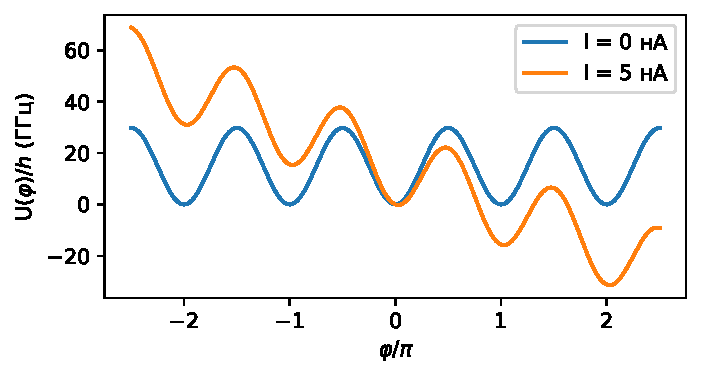
\includegraphics[width=0.7\linewidth]{Pictures/washboard}
	\caption{Потенциал ``наклонённого косинуса'', в котором происходит движение виртуальной частицы, описываемой уравнением \eqref{eq:rcsj_current}. Графики приведены для двух значений смещающего тока. Значение $E_J/h = 15$ GHz рассчитано для $I_c$ = 30 нА.}
	\label{fig:washboard}
\end{figure}

Такое уравнение можно решать классически, а в случае малых потерь и низкой температуры, пренебрегая диссипативным членом, составлять гамильтониан и квантовать его. Потенциальная энергия системы, описывающейся уравнением \eqref{eq:rcsj_current}, задается выражением (см. также \autoref{fig:washboard}):
\begin{equation}
	U(\varphi) = E_J\left(1-\cos \varphi - \frac{I}{I_c}\varphi\right).
\end{equation}
Константа $E_J$ получается из выражения для энергии идеального джозефсоновского перехода, рассчитываемого через уравнения Джозефсона и стандартное выражение для работы тока:
\begin{equation}
	U_J(\varphi) = \int_0^t V(\varphi) I(\varphi) \diff t = \frac{\hbar I_c}{2e}  \int_0^\varphi \sin\varphi \diff\varphi = E_J(1-\cos \varphi).
\end{equation}
Значение же $\omega_0$ может быть выражено через величины $E_J$ и $E_C = e^2/2C$:
\begin{equation}
	\omega_0 = \sqrt{8 E_J E_C}.
\end{equation}
Используя данную формулу можно также прояснить смысл нелинейной джозефсоновской индуктивности. Эта величина вычисляется как обратное значение второй производной энергии системы по потоку (обобщенному импульсу) $\Phi = \int_{-\infty}^{t} V(\tau) \diff \tau = \frac{\Phi_0}{2\pi} \varphi$:
\begin{equation}
	L_J = \left(\frac{\diff^2 U_J(\varphi)}{\diff \Phi^2}\right)^{-1} = \left(\frac{\diff^2 U_J(2\pi \frac{\Phi}{\Phi_0})}{\diff \Phi^2}\right)^{-1} = \frac{\Phi_0}{2\pi I_c \cos \varphi}.
\end{equation}
В пределе малых $\varphi$ индуктивность оказывается равна $\Phi_0/2\pi I_c$, и формула для $\omega_0$:
\begin{equation}
	\omega_0 = 1/\sqrt{L_J C},
\end{equation}
что совпадает с привычным выражением для частоты колебательного контура.


\subsection{Макроскопическое квантовое туннелирование}

В 1985 году Мишель Деворе, Джон Мартинис и Джон Кларк провели эксперимент \cite{devoret1985measurements}, который окончательно позволил дать ответ на вопрос, допустимо ли квантовать уравнение на макроскопическую переменную $\varphi$ в уравнении \eqref{eq:rcsj_current} (первые подобные эксперименты проводились еще в 1981 году в IBM \cite{voss1981macroscopic}). Макроскопической она является потому, что однозначно определяет экспериментально детектируемый макроскопический ток, текущий через джозефсоновский переход. Таким образом, если квантовый аналог уравнения движения для джозефсоновского перехода действительно применим, то поведение его должно совпадать с поведением квантовой частицы в потенциале \autoref{fig:washboard}. Обнаружение такого поведения в указанной работе проводилось посредством охлаждения перехода до такой низкой температуры, что термические флуктуации оказывались меньше ожидаемых квантовых флуктуаций. 
Оба типа флуктуаций приводят к тому, что частица при определенном наклоне потенциала \autoref{fig:washboard} спонтанно покидает один из его уступов, в котором находилась изначально, и начинает скатываться вниз. Это означает, что контакт переходит в резистивное состояние с ненулевым переменным напряжением, определяемым значением производной разности фаз по закону \eqref{eq:JJ2}, которое можно обнаружить в эксперименте. По вероятности, с которой частица ``убегает'' из своего уступа в единицу времени, можно определить эффективную температуру $T_\text{esc}$ эквивалентных термальных флуктуаций, вызывающих такое ``убегание''. Понятно, что при нулевой температуре классическая частица остается в покое, пока сохраняется сколь угодно маленький уступ. Однако при наличии квантовых флуктуаций $T_\text{esc}$ окажется ненулевой даже для очень низких температур образца. 

Обнаружение макроскопического квантового туннелирования в джозефсоновских системах вызвало большой интерес и споры в научном сообществе. Например, в комментарии, вышедшем через 4 года\cite{silvestrini1989comment}, результат даже оспаривался на основании необъясненного постоянного сдвига $T_\text{esc}$ для двух переходов. Однако опираясь на дополнительные результаты, которые были получены за это время, авторы ответили на критику \cite{devoret1989devoret}, отметив большую систематическую погрешность для кривой, соответствующей классическому поведению и еще раз точность данных кривой квантового перехода. Также в своем ответе авторы отмечают еще одну работу 1988 года \cite{cleland1988measurement}, содержащую результаты исследования влияния диссипации на квантовое туннелирование: выяснено было, что низкодобротные джозефсоновские переходы, специально шунтированные тонкопленочными резисторами, демонстрируют подавление макроскопического туннелирования. Также во введении к работе отмечается, что реальные динамические потери в джозефсоновском переходе, определяемые эффективным сопротивлением $R$, в сверхпроводящем режиме не  равны $R_N$ -- т.н. нормальному сопротивлению, измеряемому по наклону вольт-амперной характеристики перехода выше критического тока. В дальнейших экспериментах уже со сверхпроводящими кубитами выяснится, что собственные потери маленьких джозефсоновских переходов оказываются в действительности очень малы \cite{paik2011observation}.

Описанные эксперименты также подтолкнули обсуждение корректного квантовомеханического формализма для описания диссипативных систем \cite{caldeira1985influence, walls1985effect}. Данный вопрос представляет большой интерес не только с точки зрения практического описания джозефсоновских систем, но оказывается напрямую связан с неразрешенной до сих пор проблемой перехода от квантовомеханического микроскопического мира элементарных частиц к классическому миру макроскопических объектов, из них состоящих \cite{walls1985analysis, zurek2009quantum}.



\section{Сверхпроводниковые кубиты -- искусственные атомы}

\subsection{Очерк развития области}

После обнаружения квантовомеханического поведения такой крупной по размеру физической системы, как джозефсоновский переход, научное сообщество оказалось заинтересовано возможностью использования её в качестве элемента квантовой вычислительной системы, концепция которой родилась также в 80-х годах \cite{manin1980, feynman1982simulating}. 


\begin{figure}[t]
	\centering
	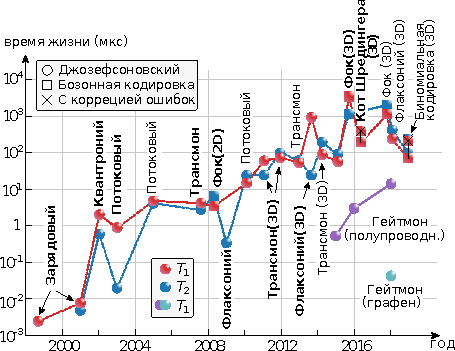
\includegraphics[width=.8\linewidth]{shoelkopfs_law.pdf}
	\caption{Иллюстрация ``закона Шелькопфа'', предсказывающего экспоненциальный рост времен релаксации и когерентности свехрпроводниковых кубитов с годами исследований. Адаптировано из обзора \cite{kjaergaard2020superconducting}. Полужирным шрифтом обозначены первые реализации указанных архитектур кубитов.}
	\label{fig:shoelkopfslaw}
\end{figure}

На самом деле уже в первых экспериментах по квантовому макроскопическому туннелированию был открыт первый сверхпроводниковый кубит -- фазовый, -- страдавший, правда, в то время от чрезвычайно быстрой релаксации при добротности измерявшихся систем не выше сотни. Несмотря на это обычно первым сверхпроводниковым кубитом называется т.н. зарядовый кубит на основе ящика куперовских пар \cite{nakamura1999coherent}, так как именно на нём в 1999 году были впервые продемонстрированы когерентные квантовые осцилляции заселенности двух состояний. Скорость релаксации в этой системе также была очень высока, поэтому для генерации импульсов товарищам Ясунобу Накамуре, Юрию Пашкину и Джао-Шеню Цаю пришлось использовать высокоскоростной цифровой генератор импульсов Anritsu MP1758A с временным разрешением порядка 5 пикосекунд -- серьезнейшую для того времени машину. 

Следом за зарядовым кубитом в 2000 году группой голландских и американских ученых был предложен и реализован потоковый кубит -- алюминиевое кольцо с тремя джозефсоновскими переходами, внешний поток через которое выставляется в $ \Phi_0/2 $ \cite{van2000quantum}. При таком внешнем потоке и ненулевой геометрической индуктивности кольца потенциал виртуальной частицы, о которой говорилось в предыдущем разделе, оказывается симметричным двухъямным с минимумами, отвечающими классическим состояниям с сверхтоками, текущими в противоположные стороны. За счет туннелирования через барьер между ямами энергетическое вырождение между классическими состояниями снимается, а основное и возбужденное состояния оказываются  ``кошками Шредингера'' -- коллективными суперпозициями большого числа частиц, доступными для измерения простыми приборами. Конечно, речь о том, чтобы приготовлять настоящих кошек в состояниях суперпозиции, не идет, так как они они являются гораздо более сложными системами и не обладают свойствами Бозе-конденсатов куперовских пар, обеспечивающими чрезвычайно слабую связь их с внешней средой. Однако и этот эксперимент, и многие другие последующие показали, что природа принципиально не запрещает суперпозиции состояний даже для очень большого числа частиц.



В 2002 году в группе ``Quantronics'' (от \textit{quantum electroninics}) Дэнисом Вионом и соавторами был реализован первый кубит, время фазовой когерентности которого приблизилось к 500 нс -- квантрониум \cite{vion2002manipulating}. Особенностью его было то, что он обладал двумя параметрами контроля частоты: напряжение на затворе, как у зарядовых кубитов на основе одноэлектронных транзисторов, и поток через контур, содержащий джозефсоновские переходы, как в потоковых кубитах. Также был реализован новый способ считывания через шунтирующий большой джозефсоновский переход, переходящий или не переходящий в резистивное состояние в зависимости от энергетического состояния кубита (в нём ни фаза, ни число куперовских пар не являются хорошо определенными переменными, и вычислительный базис строится на двух нижних собственных состояниях гамильтониана). Так как в то время еще не было полной теории, описывающей микроскопическую природу диссипации в подобных системах, в статье не указывается, какие именно решения позволили достичь увеличения времени когерентности. 

Также в 2002 году Джон Мартинис с соавторами работая в то время в Национальном Институте Стандартов и Технологии продемонстрировал когерентные осцилляции Раби на фазовом кубите \cite{martinis2002rabi} (джозефсоновский переход Nb/AlO$_x$/Nb). Когерентность кубита опять оказалась весьма низкой, порядка десятков наносекунд. Однако именно в этой работе было сделано предположение о том, что источником потерь является эквивалентный конденсатор джозефсоновкого перехода, в аморфном оксиде которого могут существовать дефекты, связывающиеся с кубитом. Интересно отметить, что примерно в то же время в Университете Канзаса проводились эксперименты на тех же кубитах, но с другим типом переходов -- NbN/AlN/NbN, и исследователи сообщали о совершенно невероятных для того времени временах когерентности в 10 мкс \cite{han2001time}, но по каким-то причинам исследования в той группе практически не продолжались.

Исследования причин потерь в джозефсоновских контактах продолжались, и в 2004 году были впервые открыты ``микроволновые резонаторы'', которые существенно уменьшали время когерентности кубитов на определенных частотах \cite{simmonds2004decoherence}. Уже тогда авторам было понятно, что скорее всего данные резонансы связаны с двухуровневыми квантовыми системами внутри перехода, хотя в строгом классическом смысле слова резонаторами такие системы назвать, конечно, было нельзя. Это открытие послужило отправной точкой для дальнейшей многолетней и кропотливой работы по подбору материалов и производственных циклов для создания сверхпроводникового квантового процессора.

Следующим шагом в экспериментах стала демонстрация так называемой квантовой электродинамики электрических цепей (\textit{circuit QED}) \cite{blais2004cavity, wallraff2004strong}. Название это было создано по образу квантовой электродинамики полостей (\textit{cavity QED}) -- области науки, впервые показавшей возможность управления изолированными одиночными квантовыми системами \cite{mabuchi2002cavity}. Архитектура, связывающая кубит с микроволновым резонатором позволяет осуществлять неразрушающее (проецирующее) измерение его состояния. Ранее такое измерение было возможно лишь для зарядовых кубитов \cite{lehnert2003measurement}, в то время как для потоковых и фазовых кубитов измерение СКВИДом было разрушающим -- приводило к нагреванию кубита и необходимости повторно инициализировать его в основное состояние. С потоковым кубитом резонатор удалось сильно связать в 2008 году \cite{abdumalikov2008vacuum}.

Квантовая электродинамика цепей открыла дорогу для новых типов кубитов. Поистине прорывным оказалось открытие в 2007 году того, что увеличение электрической емкости у сверхпроводящих островов зарядового кубита, означающее подавление зарядовой энергии в его гамильтониане, приводит к экспоненциальному подавлению зарядовой дисперсии (зависимости частот переходов между уровнями от наведенного на остров заряда) \cite{koch2007charge}. Новый тип кубита был назван трансмоном. Преодоление зарядового шума (в западной литературе встречается выражение ``life after charge noise'' \cite{houck2009life}) в свою очередь открыло новую огромную область исследований. В базе Web Of Science с момента первой публикации в 2008 году на текущий момент зарегистрировано более 450 публикаций с ключевым словом ``transmon''. Для потоковых кубитов идея шунтировать переход большой емкостью оказалась также плодотворной, позволив уменьшить зависимость от магнитного потока и, соответственно, дефазировку кубитов вызываемую потоковым шумом вне точки вырождения \cite{you2007low, yan2016flux}. Ключевая роль использования резонаторов для считывания заключается в том, что энергетические состояния трансмона, используемые в качестве вычислительного базиса, как и в фазовом кубите, оказываются неразличимы по заряду -- средний заряд на острове, шунтированном большой емкостью, оказывается нулевым как для основного, так и для возбужденного состояний. Однако эти состояния оказывается возможно различить по сдвигу частоты резонатора так же, как и в случае использования зарядовых или потоковых кубитов -- дисперсионное считывание оказалось универсальным средством.

В 2009 году был предложен очередной кубит -- т.н. флаксоний, представляющий собой контур с кинетической индуктивностью и джозефсоновским переходом \cite{manucharyan2009fluxonium}. По своей сути это ВЧ-СКВИД (сверхпроводящее кольцо с одним переходом), с тем лишь отличием, что индуктивность практически полностью набирается за счет кинетической части, реализованной при помощи цепочки джозефсоновских переходов. На таких кубитах продемонстрировано рекордное время релаксации в 8 мс при определенном значении потока за счет подавления туннелирования квазичастиц \cite{pop2014coherent}. Этот тип кубитов также поддается дисперсионному считыванию, как и предыдущие.

\subsection{Проектирование квантовых цепей на примере трансмонов}

\chapter{Автоматизация эксперимента}

\chapter{Взаимодействие двухатомной искусственной молекулы и излучения}

\chapter{Квантовый фотонный транспорт в модели Бозе-Хаббарда}

\chapter{Заключение}


\appendix
\renewcommand*\thesection{\Alph{chapter}.\arabic{section}}


\renewcommand\bibname{Список литературы}
\bibliographystyle{ugost2008}
\bibliography{dissertation.bib}
\end{document}
